\renewcommand{\tableautorefname}{tabulce}
\renewcommand{\figureautorefname}{obrázku}
\renewcommand{\subsectionautorefname}{pododdíl}
\renewcommand{\sectionautorefname}{oddíl}
\renewcommand{\chapterautorefname}{kapitole}
\counterwithout{footnote}{chapter}
\titlespacing*{\section}{0pt}{2ex plus 0.7ex minus .2ex}{1.5ex plus .2ex}
\titlespacing*{\subsection}{0pt}{1.5ex plus 0.6ex minus .2ex}{1.2ex plus .2ex}
\titlespacing*{\subsubsection}{0pt}{1.2ex plus 0.5ex minus .2ex}{1ex plus .2ex}

\chapter*{Úvod}
Lidé se odjakživa potřebují přemisťovat za účelem uspokojování svých potřeb. V~moderním světě si lidé často nevystačí pouze s~chůzí, jelikož preferují ušetřit vlastní energii i~čas. To nevyhnutelně vede k~přepravě dopravními prostředky jako je kolo, vlak nebo automobil. Ať už si člověk vybere veřejnou dopravu nebo vlastní automobil, vždy je plán dojet do správného cíle a~v~požadovaném čase. Mnohdy je však i~prioritou, aby cesta trvala co nejkratší dobu. Protože je silniční, železniční i~cyklistická síť velmi rozsáhlá, najít skutečně cestu, která trvá nejkratší možnou dobu, není snadný úkol. Je o~to komplikovanější, když je cestující závislý na spojích veřejné dopravy, které jezdí jen v~určitých intervalech.

Naštěstí existuje teorie grafů, matematický obor, který tuto úlohu -- formulovanou jako problém nalezení nejkratší cesty -- a~spoustu dalších studuje. Řešení k~těmto úlohám je typicky nalezeno více či méně sofistikovanými metodami neboli algoritmy, obvykle za pomocí výpočetní techniky.

\section*{Nalezení nejkratší cesty nejen v~dopravních sítích}
Problém nalezení nejkratší cesty se vyskytuje v~mnoha odvětvích, a~to také svědčí o~spoustě algoritmů, které byly vybudovány pro každý konkrétní problém zvlášť. Společné ale mají to, že se fyzická síť převede na abstraktní graf s~vrcholy spojené hranami, nad nimiž algoritmus provádí operace.

Algoritmy jsou využity např. pro efektivní řízení toku elektřiny po elektrické rozvodné síti \cite{SunPowerGrid}, nalezení spojení dvou lidí v~sociálních sítích \cite{RezvanianSocNetworks} nebo nalezení optimální cesty pro charaktery v~počítačových hrách \cite{XiaoPCGames}. Algoritmy nejkratších cest jsou stěžejní i~pro zprostředkování efektivní komunikace mezi zařízeními v~počítačových sítích \cite{Schwartz1980}. Hlavní roli rovněž zastávají na dopravních sítích, ať už v~navigacích řidičů v~osobní a~nákladní přepravě, v~programech dirigujících pohyb robotů v~logistických centrech či v~mobilních aplikacích vyhledávačů spojení ve veřejné hromadné dopravě (VHD). 
 
\section*{Optimalizace tras ve VHD}
V sítích veřejné dopravy je optimalizace tras a~spojů důležitá jak ze strany cestujícího, tak i~dopravce. Cestující obvykle preferuje přijet do cíle v~co nejkratším čase, protože samotná jízda je považována za neproduktivní. Dalším klíčovým faktorem je cena dopravy a~počet přestupů na trase. Vedlejší faktory jako pohodlí anebo bezpečnost také ovlivňují volby cestujícího, avšak v~menší míře. Na druhé straně je dopravce, jehož úloha je značně složitější, jelikož do rozhodovacího procesu vstupují i~další faktory, které se týkají vozidel, infrastruktury anebo personálu. Tato práce se však soustředí na tu první úlohu, tedy problém nalezení nejrychlejší\footnote{Přesněji řečeno se jedná primárně o~nalezení cesty s~\emph{nejdřívějším} příjezdem, jak bude později vysvětleno. Z~důvodu jazykové úspornosti jsou občas tyto termíny zaměňovány.} cesty v~síti VHD z~pohledu cestujícího. 

Nalezení nejrychlejší cesty na silniční síti a~nalezení optimálního spojení pro cestujícího ve VHD má mnoho společného, ale je zde kritický rozdíl. Při přepravě automobilem je možné vyjet kdykoliv, a~za předpokladu, že variace intenzity dopravy je zanedbatelná, cestovní doba bude vždy stejná. Nejrychlejší cestu lze proto převést do statického grafu, kde ohodnocení hran je neměnné. Naopak spoje ve veřejné dopravě se řídí specifickým jízdním řádem, a~tudíž den a~čas odjezdu ovlivňuje ohodnocení hran; takový graf je dynamický. A~právě vytvoření a~implementace algoritmu nejrychlejší cesty v~dynamickém grafu je cílem této bakalářské práce.

\section*{Cíl práce}
Primárním cílem tohoto textu je zdokumentovat aktuální přístupy k~návrhu algoritmických metod, které dokáží vyhledat nejrychlejší cestu mezi dvěma zastávkami\footnote{Běžný dopravní systém je multimodální, tudíž se těm místům, kde pravidelně zastavují spoje linek, říká zastávka nebo stanice dle dopravního prostředku anebo dopravního významu. Použitím jednoho ze slov se v~textu běžně myslí oba významy, nejedná-li se o~terminologický pojem.} v~systému veřejné hromadné dopravy, a~některé z~nich implementovat a~aplikovat na reálný dopravní systém. Tyto metody se dělí na grafové a~negrafové, přičemž grafovým je zde věnována větší pozornost. Detailně je popsán model grafu nazývaný \textit{stanicový model} (\textquote{Time-Dependent Model}), v~němž je pro vyhledávání využit Dijkstrův algoritmus a~jeho modifikace (TD-Dijkstra). Negrafové algoritmy pracují na odlišném způsobu a~patří mezi ně např. Connection Scan Algorithm (CSA), který je také důkladně popsán. Jak TD-Dijkstra, tak i~CSA jsou v~praktické části práce vytvořeny v~programovacím jazyce Python a~jsou aplikovány na dopravní systém Pražské integrované dopravy (PID). 

\section*{Osnova textu}
Osnova textu je klasicky rozdělena na teoretickou a~praktickou část. První kapitola se zabývá úlohou nalezení nejkratší cesty a~popisuje Dijkstrův algoritmus společně s~jeho nástavbou A*. Uvedeny jsou i~nástroje k~zrychlení těchto algoritmů.

V druhé kapitole je představen koncept časově závislých grafů. Je popsán tzv.~\textit{stanicový model} grafu, který realisticky reprezentuje skutečnou dopravní síť, na níž lze spustit TD-Dijkstru. Předposlední oddíl kapitoly se věnuje algoritmům s~negrafovou strukturou (RAPTOR, CSA), které také řeší variace úloh nejkratší cesty (popsány v~závěru kapitoly).

Třetí kapitola teoretické poznatky aplikuje na reálnou dopravní síť v~systému Pražské integrované dopravy (PID). Kapitola dokumentuje postup tvorby variací Dijkstrova algoritmu a~CSA v~programovacím jazyce Python, včetně načtení dat a~adaptace algoritmů na různé úlohy.

Ve čtvrté kapitole jsou prezentovány vlastní výsledky výkonnostních testů implementovaných algoritmů. Poslední kapitola bakalářskou práci shrnuje a~uzavírá.

\part{Teorie}
\chapter{Algoritmy nalezení nejkratší cesty}
\label{ch:algos}
V této kapitole je detailně popsán Dijkstrův algoritmus ve statických grafech, společně s~nástavbami A* a~dalšími urychlovacími (\textquote{speed-up}) technikami.

\section{Dijkstrův algoritmus}
Dijkstrův algoritmus byl vytvořený jako nástroj pro nalezení nejkratší cesty v~grafu. Byl poprvé popsán v~odborném článku z~roku 1959 nizozemským informatikem Edsgerem W. Dijkstrou, po němž je algoritmus pojmenován \cite{Dijkstra59}. Dijkstrův algoritmus dokáže nalézt nejkratší cestu z~výchozího vrcholu do všech ostatních vrcholů v~hranově ohodnoceném grafu, který může být orientovaný (pak se jedná o~digraf) nebo neorientovaný. Ohodnocení hran musí být nezáporné, aby byla zaručena správnost algoritmu. Při výskytu záporně ohodnocených hran lze použít pro nalezení nejkratší cesty např. Bellmanův-Fordův algoritmus. Dijkstrův algoritmus je schopný řešit dva typy problémů nejkratších cest, a~to jak z~počátku do jednoho vrcholu (cíle), tak z~počátku do všech ostatních vrcholů. Nejkratší cestou se většinou myslí to první, zatímco to druhé se někdy nazývá strom nejkratších cest.

\subsection{Definice a~popis algoritmu}
Nechť je dán orientovaný graf $G = (V, E)$, kde $V$ je množina všech vrcholů grafu $G$ a~$E$ je množina všech hran grafu $G$. Každá hrana $(u,v) \in E$ má nezápornou délku $L(u,v)$. Cílem algoritmu je nalézt nejkratší cestu z~počátečního vrcholu $s$ do každého vrcholu v~množině cílových vrcholů. V~případě, že je cílový vrchol pouze jeden, je tento vrchol označen jako $t$. Délka nejkratší cesty z~vrcholu $v$ do vrcholu $w$ je značena $d(v,w)$.

Při postupu algoritmem se vrchol vyskytuje v~právě jednom ze tří stavů: \textit{nedosažený}, \textit{dosažený} a~\textit{probraný}\footnote{V literatuře je možně se setkat i~s~jinými názvy: (nenalezený, otevřený, uzavřený) či (nenavštívený, navštívený, prozkoumaný), ale jedná se pouze o~stylistickou preferenci autora.}, kde dosažený vrchol je neprobraný. Vrcholy jsou postupně ohodnoceny číslem $E(v)$ (z~ang. \textquote{estimation}), které udává horní odhad nejkratší cesty z~počátku $s$ do vrcholu $v$. Na konci výpočtu je to přímo vzdálenost mezi $s$ a~$v$ \cite{mffDijkstraKucera}. Ohodnocení vrcholů v~jednotlivých stavech je pak následující:

\begin{description}
	\item[Nedosažený vrchol] Vrchol zatím nebyl ohodnocen, proto $E(v) = \infty$ (nebo též někdy $E(v)$ není definováno).
	\item[Dosažený vrchol] Vrchol, který byl v~průběhu algoritmu prozkoumán a~jehož ohodnocení je reálné číslo, nicméně ale ještě nebyl definitivně ohodnocen.
	\item[Probraný vrchol] Vrchol, jehož ohodnocení $E(v)$ udává definitivní (nejkratší možnou) vzdálenost z~počátku $s$ do vrcholu $v$. 
\end{description}

Vrcholy, které jsou dosažené ale neprobrané, jsou zařazeny do prioritní fronty, jejíž první prvek je vrchol s~nejnižším ohodnocením. Pro probrané i~dosažené vrcholy $v$ je navíc dán vrchol $P(v)$ (předchůdce), pomocí něhož bude možné dohledat cestu o~délce $E(v)$.

{\normalsize
\colorbox{gray!10}{%
\begin{minipage}{0.95\textwidth}
\vspace{0.5em}
\begin{minipage}[t]{0.98\textwidth}
		
		Postup Dijkstrova algoritmu je dán následujícími kroky \cite{mffDijkstraKucera}:
		\begin{enumerate}
			\item[] \textcolor{darkgray}{\small // označ všechny vrcholy jako \textit{nedosažené}}
		\item pro všechna $v \in V$ označ $E(v) := \infty$, $P(v) := \text{není definováno}$ 
		\item počátek $s$ označ jako \textit{dosažený} a~$E(s) := 0$
		\item dokud existují \textit{dosažené} vrcholy, opakuj:
		\begin{enumerate}[label ={\normalfont\itembox(0.1em)(0.1em){\arabic{enumi}.\arabic*}}]
			\item[] \textcolor{darkgray}{\small // vyber z~prioritní fronty první prvek}
			\item zvol \textit{dosažený} vrchol $u$ takový, kde $E(u) \leq E(w)$ pro všechny ostatní \textit{dosažené} vrcholy $w$
			\item označ $u$ jako \textit{probraný}		
			\item[] \textcolor{darkgray}{\small // prozkoumej sousedy a~zkontroluj, jestli nová cesta má menší ohodnocení}
			\item pro každý vrchol $w$, pro který existuje hrana $(u,w) \in E$ a~platí $E(u) + L(u,w) < E(w)$:
			\begin{enumerate}[label = {\normalfont\arabic{enumi}.\arabic{enumii}.\arabic*}]
				\item pokud je vrchol $w$ \textit{nedosažený}, označ jej jako \textit{dosažený}
				\item[] \textcolor{darkgray}{\small // nastav nové ohodnocení vrcholu a~zaznamenej předchůdce}
				\item označ $E(w) := E(u) + L(u,w)$, $P(w) := u$
			\end{enumerate}
		\end{enumerate}
		\item ukonči algoritmus
	\end{enumerate}
\end{minipage}

\vspace{0.5em}
\end{minipage}%
}}

Pokud je po skončení algoritmu cílový vrchol $t$ probraný, $E(t)$ je délka nejkratší cesty. V~opačném případě nejkratší cesta v~grafu mezi $s$ a~$t$ neexistuje.~U úlohy nalezení cesty z~\(s\) do \(t\) lze algoritmus ukončit dříve, a~to tehdy, když je z~prioritní fronty vybrán \(t\). Cíl \(t\) je totiž nyní definitivně ohodnocen, a~tak kratší cestu do tohoto vrcholu již nelze najít.

Pro nalezení konkrétní cesty včetně všech mezilehlých vrcholů je nutno postupovat od cíle do počátku podle hodnot $P(w)$. $P(w)$ udává předchůdce vrcholu $w$ na nejkratší cestě. Při zpětném průchodu se jedná o~následovníka. 

{\normalsize
\colorbox{gray!10}{%
\begin{minipage}{0.95\textwidth}
\vspace{0.5em}
\begin{minipage}{0.98\textwidth}
	
	Postup nalezení kompletního seznamu vrcholů na nejkratší cestě je dán \cite{mffDijkstraKucera}:
	\begin{enumerate}
		\item vytvoř prázdný seznam $S$
		\item[] \textcolor{darkgray}{\small // začni procházet od cílového vrcholu}
		\item nastav $w := t$ a~vlož $t$ na začátek seznamu $S$
		\item[] \textcolor{darkgray}{\small // pokračuj, dokud existuje předchůdce vrcholu v~původním grafu}
		\item dokud $P(w) \neq \text{není definováno}$:
		\begin{enumerate}[label ={\normalfont\itembox(0.1em)(0.1em){\arabic{enumi}.\arabic*}}]
			\item vlož $P(w)$ na začátek seznamu $S$
			\item $w := P(w)$
		\end{enumerate}
		\item ukonči algoritmus
	\end{enumerate}
	\end{minipage}
	\vspace{0.5em}
\end{minipage}%
}}

Neprázdný seznam $S$ obsahuje výčet probraných vrcholu nejkratší cesty, včetně počátku $s$ a~cíle $t$.

Dijkstrův algoritmus běží rychlostí $O(|E|\cdot log|V|)$, když se k~výběru vrcholů ze seznamu použije prioritní fronta a~binární halda \cite{ericksonShortestPaths}. Správnost algoritmu je dokázána v~původní Dijkstrově publikaci anebo v~\cite{mffDijkstraKucera}.

\section{A*}
\label{staticASTAR}
A* (A~star) algoritmus je nástavba Dijkstrova algoritmu, která byla poprvé popsána v~roce 1968 \cite{HartAstar}. Liší se tím, že při procházení vrcholů v~grafu je ohodnocení vrcholů určeno funkcí $f(v) = g(v) + h(v)$. Jako u~Dijkstrova algoritmu, $g(v)$ udává vzdálenost vrcholu $v$ od počátečního vrcholu, navíc zde však figuruje heuristická funkce $h(v)$, která udává dolní odhad nejkratší cesty z~vrcholu $v$ do cíle. Cílem využití heuristiky je \textquote{usměrnění} algoritmu, tj.~při prohledávání upřednostňovat vrcholy, které jsou blíže k~cíli, a~ignorovat ty, které se od něj vzdalují.

Obecně platí, že přesnější heuristika (dolní odhad je blízko skutečné vzdálenosti) činí algoritmus efektivnějším. Je zřejmé, že pokud dolní odhad $h(v) = 0$, tak ekvivalentní zápis ohodnocení vrcholů by byl $f(v) = g(v)$ a~jednalo by se tak o~standardní Dijkstrův algoritmus. Při nenulové heuristické funkci je nutné zajistit, aby $h(v)$ byla přípustná a~monotónní.

\begin{description}
	\item[Přípustná funkce] Funkce $h(v)$ se nazývá přípustná, právě tehdy když $h(v) \leq d(v, t)$ pro každý vrchol grafu \cite{dechter1985generalized}.
\end{description}

Přípustná funkce nikdy nepřeceňuje opravdovou vzdálenost od daného vrcholu do cíle. Pokud je funkce přípustná a~zároveň monotónní (viz níže), algoritmus A* zaručeně nalezne optimální cestu \cite{Edelkamp05}.

Intuitivní nástin důkazu přípustnosti za předpokladu monotonie: Nechť v~grafu existuje unikátní nejkratší cesta \(P\) o~délce \(d(s,t)\) a~vrchol \(v\), který neleží na \(P\). Vrchol \(v\) může být nedosažený, dosažený, nebo probraný. Optimalita musí být dokázána pro každý stav vrcholu zvlášť a~pro všechny takové vrcholy \(v\). Zaprvé pokud je \(v\) probraný a~neleží na \(P\), tak je optimalita zaručena ze stejného důvodu jako u~Dijkstrova algoritmu.

Zadruhé je \(v\) dosažený. U~takového vrcholu platí, že nebyl vybrán z~prioritní fronty, a~tak \[d(s,t) < g(v) + h(v).\] Za předpokladu, že by \(v\) mělo ležet na $P$, muselo by platit \[d(s,t) > d(s,v) +d (v,t).\] Vyřešením soustavy nerovnic a~$g(v) = d(s,v)$ plyne, že $h(v) > d(v,t)$, tedy že dolní odhad je větší než skutečná vzdálenost. Ovšem platí-li $h(v) \leq d(v,t)$ (dolní odhad je přípustný), situace, že \(v\) je dosažený a~má ležet na \(P\), nemůže nastat.

Zatřetí je vrchol \(v\) nedosažený. U~něj \(g(v) = \infty\) a~optimalita opět plyne z~Dijkstrova algoritmu. 

A tak pokud $\forall v\in V,\, h(v) \leq d(v,t)$, je zaručeno, že optimální cesta \(P\) o~délce \(d(s,t)\) byla nalezena. Formálně dokázáno např. v~\cite{PearlHeuristics}. Na \autoref{pripustnost} je graficky znázorněno, proč nepřípustná funkce nemusí vždy vést k~nalezení optimálního řešení.

% Intuitivní nástin důkazu: Pokud v~grafu existuje unikátní cesta o~délce $d(s,t)$, na které neleží vrchol $v$ a~$v \neq t$, znamená to, že $d(s,t)$ < $g(v) + h(v)$. Vrchol $v$ tak není probraný, protože algoritmus byl ukončen dříve. Pokud by $d(s,t)$ měla $v$ procházet, muselo by platit $d(s,t) > d(s, v) +d (v,t)$. Vyřešením soustavy nerovnic a~$g(v) = d(s,v)$ plyne, že $h(v) > d(v,t)$, tedy že dolní odhad je větší než skutečná vzdálenost a~vrchol $v$ nebyl navštíven. Ovšem platí-li $\forall v~\in V,\, h(v) \leq d(v,t)$, pak dolní odhad je přípustný a~každá optimální cesta bude prozkoumána. Formálně dokázáno např. zde \cite{PearlHeuristics}. Na \autoref{pripustnost} je graficky znázorněno, proč nepřípustná funkce nemusí vždy vést k~nalezení optimálního řešení.

\begin{figure}[htbp]
	\centering
	\begin{subfigure}[b]{1\textwidth}
		\centering
		\pripustnostOne
		\caption{Počáteční fáze algoritmu. Heuristická funkce u~vrcholu \(a\) přeceňuje odhad délky do cíle \(t\) o~dvě jednotky (6 namísto 4).}
        \label{pripustnostOne}
	\end{subfigure}

	\vspace{1em}
	
	\begin{subfigure}[b]{1\textwidth}
		\centering
		\pripustnostTwo
		\caption{Konečný stav algoritmu. Vrcholy jsou probrány v~pořadí \(s, b, c, t\). Protože je vrchol \(t\) definitivně ohodnocen, algoritmus je předčasně ukončen. Optimální cesta přes \(a\), která je kratší o~jednu jednotku (11 namísto 12), nebyla prozkoumána.}
        \label{pripustnostTwo}
	\end{subfigure}

	\caption[Porušení podmínky o~přípustnosti vede k~suboptimálnímu výsledku A*.]{Příklad grafu, ve kterém je A* algoritmus ukončen dříve, než je nalezena nejkratší cesta, protože je porušena podmínka o~přípustnosti. Probrané vrcholy jsou označeny tučně. Ohodnocení vrcholu je v~\textcolor{gray}{šedém} ovále dáno součtem délky cesty do vrcholu a~heuristické funkce \(h(v)\).}
	\label{pripustnost}
\end{figure}

Dále musí být splněna podmínka o~monotonii neboli konzistenci.

\begin{description}
	\item[Monotónní funkce] Funkce $h(v)$ je monotónní (nebo též konzistentní), pokud v~grafu pro každý pár vrcholů $v$ a~$w$ platí:
	$$
	h(v) \leq d(v,w) + h(w).
	$$
\end{description}

Tato vlastnost říká, že odhad délky nejkratší cesty z~vrcholu $v$ nesmí být větší než součet délky hrany $(v,w)$ a~odhadu ve vrcholu $w$. Jednoduše to znamená, že odhad nejkratší cesty z~$v$ do cíle za podmínky, že cesta prochází $w$, nesmí být menší než bez této podmínky \cite{PearlHeuristics}. Jedná se tak o~trojúhelníkovou nerovnost, která zajištuje, že jakmile je vrchol probraný, není potřeba jej znovu navštěvovat; algoritmus se tak stává efektivnějším. Monotonie implikuje přípustnost \cite{PearlHeuristics}. 

\subsection{Základní heuristiky}
Typická přípustná i~monotónní heuristická funkce je Eukleidovská metrika, která v~rovině udává přímou vzdálenost mezi dvěma body (tj.~vzdálenost vzdušnou čarou):
$$
d(X, Y) = \sqrt{(x_1 - y_1)^2 + (x_2 - y_2)^2},
$$
kde \(X\text{ a~} Y\) jsou body a~\(x_i \text{ a~} y_i\) jsou jejich souřadnice.

V určitých situacích, kde je pohyb dovolen pouze čtyřmi směry (např. labyrint ve čtvercové síti nebo síť pravoúhlých ulic), je výhodnější použít Manhattanskou metriku. Ta měří vzdálenost mezi dvěma body jako součet rozdílů souřadnic na každé ose. Rozdíly jsou v~absolutní hodnotě. V~porovnání s~Eukleidovskou metrikou bude v~mřížkové síti Manhattanská metrika přesnější, protože její odhad skutečné vzdálenosti je stejný nebo vyšší, aniž by byla porušena podmínka o~přípustnosti. 

\subsection{Landmarky (ALT)}
\label{staticLANDMARKS}

Zajímavou alternativou ke standardním metrikám výše je využití tzv.~landmarků (z~ang. význačné nebo orientační body). Heuristika byla v~této formě poprvé popsána Goldbergem a~Harrelsonem \cite{goldberg03AMeetsGT} a~využívá k~určení dolního odhadu trojúhelníkovou nerovnost. Algoritmy využívající tuto metodu se proto nazývají ALT algoritmy, jelikož vychází z~\textbf{A}* algoritmu a~pro výpočet využívají \textbf{L}andmarky a~\textbf{T}rojúhelníkovou nerovnost.

Nechť existuje landmark $L$, k~němuž existuje nejkratší cesta o~délce $d(v,L)$ z~vrcholu $v$. Poté z~trojúhelníkové nerovnosti plyne, že $d(v,w) + d(w,L) \geq d(v,L)$. Úpravou $d(v,w) \geq d(v,L) - d(w,L)$. Dosazením $w = t$ lze získat $d(v,t) \geq d(v,L) - d(t,L)$.

Podobně pokud existuje nejkratší cesta o~délce $d(L,v)$ od \(L\) do vrcholu \(v\), platí $d(L,v) + d(v,w) \geq d(L,w)$. Úpravou $d(v,w) \geq d(L,w) - d(L,v)$ a~dosazením $w = t$ pak $d(v,t) \geq d(L,t) - d(L,v)$. Heuristika \(h(v) = d(v,t)\) je poté minimum z~těchto dolních odhadů.

\begin{figure}[htbp]
	\centering
	\trojuhelnikovaNerovnost
	\caption[Princip trojúhelníkové nerovnosti ALT algoritmu.]{Princip trojúhelníkové nerovnosti ALT algoritmu v~grafu se známou délkou trasy do landmarku (\textcolor{BlueViolet}{modře}). Vrcholy \(v, t \text{ a~} L\) tvoří trojúhelník z~orientovaných hran. Nejkratší cesta z~\(v \text{ do } L\) je dlouhá 9~jednotek (j), z~\(t \text{ do } L\) je dlouhá 5~j. Z~trojúhelníkové nerovnosti platí, že \textcolor{RedOrange}{oranžová} cesta z~\(v \text{ do } t\) je dlouhá alespoň 4~j; tento případ nastane právě tehdy, když cesta z~\(v \text{ do } L \text{ prochází vrcholem } t\) (zaznačeno čárkovaně).}
	\label{pic:trojuhelnikovaNerovnost}
\end{figure}

\renewcommand{\figureautorefname}{obrázek}
Jinými slovy dolní odhad vzdálenosti nejkratší cesty je rozdíl vzdálenosti od aktuálního vrcholu k~landmarku a~od cíle k~landmarku, nebo rozdíl vzdálenosti od landmarku k~cíli a~od landmarku k~aktuálnímu vrcholu (pro první případ viz \autoref{pic:trojuhelnikovaNerovnost}). Protože jsou hrany orientované, je nutné rozlišovat tyto dvě rovnice. V~případě neorientovaného grafu by bylo možné jednu rovnici nahradit vložením druhé rovnice do absolutní hodnoty.

Pokud je landmarků více, existuje několik takových dolních odhadů. Žádný odhad nepřeceňuje opravdovou vzdálenost, a~tak z~nich je nejlepší zvolit ten maximální odhad, protože je nejpřesnější. 
\renewcommand{\figureautorefname}{obrázku}

Ačkoliv ALT algoritmy jsou rychlé \cite{bauer2011experimental}, nevýhoda tohoto přístupu vězí v~tom, že je nutno předem spočítat pro každý prvek z~množiny vrcholů grafu nejkratší cestu od i~do každého prvku v~množině landmarků. Tyto cesty stačí vypočítat pouze jednou, a~tak nejsou součástí každého spuštění algoritmu; výpočet se provede před počátečním spuštěním ve fázi předzpracování (\textquote{pre-processingu}). V~obrovských grafech sice může tato fáze trvat až několik hodin, ale nejkratší cesta mezi dvěma body na silniční sítí se jen zřídkakdy mění, proto vzdálenosti od předzpracovaných landmarků zůstávají věrohodné po poměrně dlouhou dobu.

\subsubsection{Výběr landmarků}
Důležitým aspektem pro tuto heuristiku je výběr landmarků. V~původním článku byly navrhnuty metody \textit{random}, \textit{planar} a~\textit{farthest} \cite{goldberg03AMeetsGT}. K~nim se pak přidaly metody \textit{avoid} a~\textit{maxCover} \cite{goldberg05PointToPoint}.

\textit{Random} metoda je pouze náhodný výběr; je to nejrychlejší metoda, ale není příliš efektivní. \textit{Planar} využívá znalosti, že silniční síť je geometrický graf, ve kterém délky hran silně korelují se vzdáleností. K~nalezení landmarků se graf rozdělí na několik stejně velkých výseků kružnice se středem v~centrálním uzlu sítě. Poté je iterativně v~každém výseku nalezen takový uzel, který je od centrální nejvzdálenější; je-li blízko hranice s~jiným výsekem, je uzel přeskočen.

U~metody \textit{farthest} je rovněž snaha nalézt co nejvzdálenější uzly. První landmark je zvolen náhodně, zatímco každý další je pak zvolen tak, aby od všech ostatních landmarků byl co nejdále. Několik optimalizací výběru blíže popisuje Goldberg a~Harrelson \cite{goldberg03AMeetsGT}, jako například opětovné odstranění již vybraných landmarků pro maximalizaci vzájemných vzdáleností.

Metoda \textit{avoid} funguje na té bázi, že se landmark vloží na místo, které aktuálně není dobře pokryto landmarky. U~takového místa platí, že dolní odhad je oproti skutečné vzdálenosti příliš malý, a~je tam tedy vhodné landmark umístit. Nejsložitější ale zato nejefektivnější je způsob výběru \textit{maxCover}, kde je snaha zvolit landmarky tak, aby pro co největší počet vrcholů platilo, že skutečná vzdálenost mezi dvěma vrcholy je právě ta hodnota získána výpočtem vůči alespoň jednomu landmarku. Řešení je vylepšováno iterativně zkoušením několika kandidátských landmarků až je nakonec dosaženo lokální optimum \cite{goldberg05PointToPoint}.

\section{Další speed-up techniky Dijkstrova algoritmu}
Speed-up technikami se myslí úpravy, pomocí kterých je možno zrychlit průběh základního Dijkstrova algoritmu. Typicky se jedná o~techniky, které eliminují počet vrcholů, které musejí být prozkoumány. Velikost grafu je tak snížena a~rychlost vyhledávání zvýšena. A* je také jedna ze speed-up technik.

\subsection{Oboustranné vyhledávání}
\label{sec:oboustranvyhl}
Zásadní technikou pro zrychlení, která se využívá u~většiny pokročilých algoritmů, je oboustranné vyhledávání \cite{bauer2011experimental}. U~standardního Dijkstra algoritmu je graf $G$ prohledáván pouze z~počátku do cíle, avšak u~oboustranného vyhledávání je tomu tak i~z~cíle do počátku, akorát v~obráceném grafu $G$, ve kterém je orientace hran obrácena.\footnote{Jednoduše řečeno pro každou orientovanou hranu \{u,v\} v~grafu \(G\) platí, že v~obráceném grafu to bude hrana \{v,u\}.} Když je první vrchol $v$ dosažen z~obou směrů, k~ukončení algoritmu ještě nutně nedochází, ale znamená to, že horní odhad $\mu$ nejkratší cesty je nyní vzdálenost od počátku do $v$ a~od cíle do $v$. Pokaždé, když je v~dopředném i~zpětném vyhledávání dosažen totožný vrchol (klidně i~vícekrát), je zkontrolováno, jestli odhad $\mu$ není nižší. Pokud je, tak se \(\mu\) aktualizuje. 

\begin{description}
	\item[Podmínka ukončení] Algoritmus je ukončen, jakmile je v~obou prioritních frontách na prvním místě vrchol, jejichž součet je alespoň tak velký jako $\mu$.
\end{description}

Podmínku ukončení si lze intuitivně představit tak, že každá nová prozkoumaná hrana nikdy nemůže vytvořit cestu, která by byla menší než $\mu$, protože každý vrchol z~fronty musí být spojen s~vrcholem, který ještě nebyl dosažen anebo probrán. V~obou případech bude $\mu$ překročeno. A~tak cesta o~délce $\mu$ musí být nejkratší cestou v~grafu.

\renewcommand{\figureautorefname}{obrázek}
\subsection{Arc-Flags}
Další z~metod je, podobně jako ALT, náročná na předzpracování, nicméně vyhledávání dotazů cest trvá velmi krátkou dobu \cite{bauer2011experimental}. Metoda byla poprvé popsána Lautherem \cite{lauther05Arcs}, na kterou později navazuje akcelerovaná verze \cite{kohler2005acceleration}. Princip Arc-Flags nebo česky \textquote{označení hran} vychází z~předpokladu, že je možné vyřadit hrany během vyhledávání, pokud hrana určitě nenáleží nejkratší cestě. Tento přístup využívá graf $G$ rozdělený na několik regionů $R_1\ldots R_k$, kde každý vrchol náleží právě jednomu regionu. Každá hrana nese $k$ označení. Označení hrany nabývá hodnoty \texttt{TRUE} na pozici $i$ (pro region $R_i$), pokud hrana náleží nejkratší cestě alespoň do jednoho vrcholu v~$R_i$ anebo pokud hrana leží v~$R_i$; jinak nabývá \texttt{FALSE} (viz \autoref{pic:arc_flags}).
\renewcommand{\figureautorefname}{obrázku}

\begin{figure}[htbp]
	\centering
	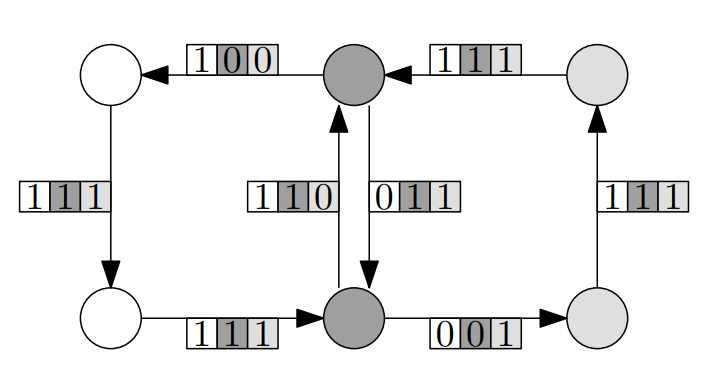
\includegraphics[width = 0.8\textwidth]{arc_flags}
	\caption[Ukázka ohodnocení hran metodou Arc-Flags.]{Ukázka ohodnocení hran metodou Arc-Flags v~grafu se třemi barevně odlišenými regiony. Hrana má označení 1 (\texttt{TRUE}) u~té barvy regionu \(R\) právě tehdy, když se v~\(R\) nachází anebo leží na nejkratší cestě do alespoň jednoho vrcholu v~\(R\). Převzato z~\cite{Delling2009enginneringRoute}.}
	\label{pic:arc_flags}
\end{figure}

Ve fázi předzpracování je nutné pro každou hranu, která je na hranici regionu $R_i$, najít strom nejkratších cest. Pokud je původní graf $G$ orientovaný, je strom nalezen v~obráceném grafu $G_{rev}$. Všechny hrany náležící stromu nejkratších cest jsou pak označeny \texttt{TRUE} na pozici $i$. Jakmile jsou všechny hraniční hrany takto označeny, Dijkstrův algoritmus při vyhledávání může vyřadit všechny hrany, které zaručeně nevedou do regionu, ve kterém se nachází cíl. V~tomto cílovém regionu je pak postupováno standardním způsobem. Nabízí se však metody několika úrovňového rozdělení (sub-regiony), které tuto konečnou fázi algoritmu opět zrychlí za cenu delšího předzpracování \cite{mohring2005partitioning}. Heuristiky efektivního rozdělení regionů uvádějí např. Hilger et al. \cite{hilger2008fast}.

\subsection{Highway Hierarchies}
Existuje nespočet dalších technik pro urychlení základního Dijkstra algoritmu, které se navíc dají mezi sebou různě kombinovat. Za zmínku ještě stojí skupina algoritmů, které člení graf do více úrovní a~vytváří jakousi hierarchii \cite{sanders05HHHasten}. 

Prvním z~nich je \textquote{Highway Hierarchies}, který využívá intuitivní myšlenky, že při cestování na dlouhé vzdálenosti jsou dálnice mnohem důležitější než silnice II.~a~III. tříd nebo místní komunikace. Tyto silnice jsou důležité pouze v~malé oblasti kolem počátku a~cíle cesty. Tato metoda tak převádí graf do několika úrovní, které volně pasují na výše zmíněné typy silnic, nicméně úrovní v~grafu může být o~mnoho více a~nevyžadují manuální kategorizaci silnic.

\begin{figure}[htbp]
	\centering
	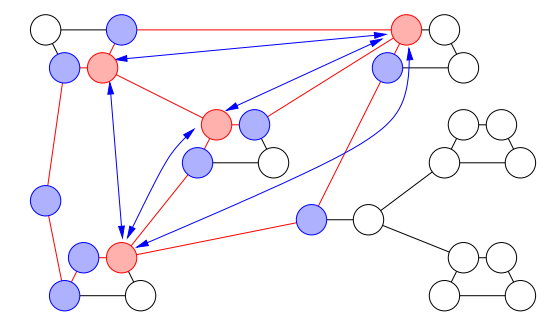
\includegraphics[width = 0.8\textwidth]{highway}
	\caption[Vytvoření zkrácené sítě dálnic metodou Highway Hierarchies.]{Vytvoření zkrácené sítě dálnic metodou Highway Hierarchies. Hrany zaznačeny \textcolor{red!75}{červeně} jsou součástí dálniční sítě. \textcolor{blue!75}{Modré vrcholy} jsou zkráceny a~\textcolor{blue!75}{modré hrany} značí zkratky. Převzato z~\cite{SchultesHHMaster}.}
	\label{pic:highway}
\end{figure}

Formálněji, graf je opět rozdělen na několik lokálních regionů neboli sousedství \cite{sandersEnginneringHH}. Není-li počátek a~cíl ve stejném lokálním regionu, je možné najít takové hrany, které se nacházejí na nejkratší cestě. Tyto hrany jsou tzv.~\textquote{highway} hrany. Z~vrcholů těchto hran se vytvoří maximální vrcholově indukovaný podgraf se stupněm každého vrcholu alespoň dva.\footnote{Takový podgraf, ve kterém platí, že každý pár vrcholů je v~podrafu spojen hranou právě tehdy, když je spojen i~v~původním grafu. Počet takových vrcholů je v~grafu maximální a~zároveň každý z~nich má stupeň alespoň dva.} V~podgrafu se pak zruší každý vnitřní vrchol $v$ (vrchol se stupněm právě dva), který sousedí s~vrcholy $u$ a~$w$, společně s~hranami s~$v$ incidujícími. Pro zachování struktury jsou tyto hrany nahrazeny jednou novou hranou, jejíž délka je rovna zrušeným incidujícím hranám. Tímto zkrácením (kontrakcí) se vytvoří zkrácená síť dálnic (\textquote{contracted highway network}) jako na \autoref{pic:highway}.



\subsection{Contraction Hierachies}
\label{staticCH}
Další metoda, vyvinuta primárně Geisbergerem, navazuje právě na ten poslední krok minulého algoritmu, tedy na zkracování (kontrakci) nepotřebných vrcholů a~nahrazování hran zkratkami; metoda se proto jmenuje \textquote{Contraction Hierarchies} \cite{geisberger2008CHDiploma, geisberger2008CHFaster}.\footnote{Zajímavý ilustrativní průvodce je v~\cite{lazarsfeldGuide}.} U~této metody je navíc specifické, že vytváří hierarchii \emph{všech} vrcholů v~grafu podle pořadí, v~jakém byly zkráceny. Je-li pořadí efektivně zvoleno, budou dříve zkracované vrcholy méně důležité (jako např. křižovatka se slepou ulicí), zatímco ty později zkracované budou hrát větší dopravní úlohu. 

Zkracování probíhá následovně: když je vrchol $v$ zkracován, jsou prověřeny nejkratší cesty mezi všemi páry sousedů $v$. Pokud nejkratší cesta mezi dvěma sousedy $u$ a~$w$ vede jen a~právě přes $v$, je vytvořena nová hrana, tzv.~zkratka. Není-li $v$ na nejkratší cestě (existuje tzv.~\textquote{witness} cesta), hrany jsou zrušeny bez náhrady. Například na \autoref{pic:contraction} byly při zkracování vrcholu $v$ celkově zrušeny čtyři hrany a~dvě byly přidány.

\begin{figure}[htbp]
	\centering
	\begin{subfigure}[b]{0.45\textwidth}
		\centering
		\contractionOne
		%\caption{}
        \label{contraction_1}
	\end{subfigure}
	\hfill
	\begin{subfigure}[b]{0.45\textwidth}
		\centering
		\contractionTwo
		%\caption{}
        \label{contraction_2}
	\end{subfigure}

	\caption[Zkrácení vrcholu v~grafu metodou Contraction Hierarchies.]{Zkrácení vrcholu \(v\) v~grafu metodou Contraction Hierarchies. Vlevo je původní graf, vpravo je stav po zkrácení. Čárkovaně jsou zaznačeny zrušené hrany a~vrchol \(v\). \textcolor{RedOrange}{Oranžovou} jsou vyznačeny hrany (zkratky), které musí být kvůli zkrácení vytvořeny.}
	\label{pic:contraction}
\end{figure}

Takto jsou postupně zkráceny všechny vrcholy grafu. Ideální je při zkracování postupovat od těch vrcholů, kde rozdíl zrušených a~nově vytvořených hran je co největší, aby graf nerostl na velikosti. Některé heuristiky zrychlení tohoto procesu jsou popsány Geisbergerem a~dalšími autory v~\cite{geisberger2008CHDiploma, geisberger2008CHFaster}.

Pro vyhledání nejkratší cesty u~orientované grafu \(G\) pokračuje algoritmus tak, že postupně v~dopředném směru od počátku skenuje podgraf \(G\), který obsahuje orientované hrany mezi $v$ a~$w$, pokud byl $v$ zkrácen před $w$. Zároveň zpětný algoritmus skenuje orientované hrany mezi $v$ a~$w$, pokud byl $v$ zkrácen po $w$, a~to v~obráceném grafu \(G\). Jinými slovy oba algoritmy \textquote{stoupají} v~hierarchii vrcholů, dokud není splněna podmínka ukončení \cite{geisberger2008CHDiploma} (viz \autoref{sec:oboustranvyhl}).

Pro získání přesné cesty je pak nutné rekurzivně rozbalit jednotlivé zkratky, kde každá z~nich postupně obsahuje nejpozději zkrácený vrchol.

\noindent\rule[0.5ex]{\linewidth}{1pt}

Madkour et al. uvádějí soupis mnoha dalších algoritmů ve statických i~dynamických grafech, které obsahují algoritmy jako např. Transit-Node Routing nebo Hub Labeling, v~této publikaci \cite{madkour2017survey}; Delling et al. pak v~této \cite{Delling2009enginneringRoute}.

\chapter{Nalezení nejrychlejší cesty v~jízdních řádech: modely a~algoritmy}

V minulé kapitole byly představeny algoritmy a~specifické speed-up techniky pro nalezení nejkratší cesty ve statických grafech. V~této kapitole je uveden koncept časově závislých grafů. Ty dovolují pracovat s~údaji v~jízdních řádech: čas odjezdu a~příjezdu a~zastávka odjezdu a~příjezdu spoje. Dále jsou představeny nástavby na již uvedené algoritmy a~heuristiky, které umožní převést statická data na dynamická.

\section{Úvod do časově závislých grafů}

Grafy lze rozdělit na dva typy: statické a~dynamické grafy. U~statických grafů je množina hran a~vrcholů během výpočtu stejná a~také zůstává neměnné ohodnocení hran. Dynamické grafy se dělí na ty, u~kterých se mění počet vrcholů nebo hran (např. evoluční graf sociální sítě \cite{tejaDynamic}), a~na ty, u~kterých je ohodnocení hran v~čase proměnlivé. K~modelování veřejné hromadné dopravy je vhodné využít ten druhý typ dynamického grafu, který se nazývá \textit{časově závislý graf}.

Typicky časově závislým systémem je silniční síť, a~to především ve velkých městech a~na dálnicích. Rychlost vozidel je inverzně závislá na hustotě dopravního proudu, která je během dne proměnlivá. Hustota bývá v~ranní a~odpolední špičce zpravidla nejvyšší, tudíž rychlost je nejnižší. V~grafu se to projevuje odlišným hranovým ohodnocením – představujícím dobu potřebnou k~projetí úseku – během dne. Proto je nutno při vyhledání nejrychlejší cesty s~touto proměnlivostí počítat; algoritmus musí reagovat na to, v~jaký den a~hodinu má být cesta uskutečněna a~podle toho najít optimální řešení. Ohodnocení hran si tak nevystačí s~konstantou jako u~statických grafů, nýbrž je nutné zavést funkci $F(\tau)$, kde $\tau$ je čas, v~jaký je hrana využita k~přejezdu. 

\subsection{Časově závislé grafy pro veřejnou dopravu}
\label{casoveZavGrafy}
Přejezd přes hranu v~grafu sítě VHD také není konstatní. Oproti silniční síti lze ohodnocení hran vyčíst přímo z~jízdního řádu, za předpokladu, že na trase nedochází ke zpoždění. Základní myšlenka tvorby ohodnocení hran následuje po několika terminologických definicích.

Jízdní řád obsahuje seznam spojů, které začínají ve výchozí a~končí v~koncové stanici (zastávce). Spoj obvykle obsahuje i~mezilehlé stanice. Převedením jízdního řádu do grafu vznikají vrcholy a~hrany. Vrcholy jsou jednotlivé stanice, které jsou spojeny hranou, existuje-li mezi nimi elementární spojení (nazýváno též jen \textit{spojení}). Elementární spojení $c$ je definováno pěticí atributů:
\[
(c_{\text{odj\_st}},\, c_{\text{prij\_st}},\, c_{\text{odj\_}\tau},\, c_{\text{prij\_}\tau},\, c_{\text{spoj\_id}}),
\]
po řadě stanice odjezdu, stanice příjezdu, čas odjezdu, čas příjezdu a~unikátní identifikační číslo spoje.

Mezi stanicemi, mezi kterými není žádné spojení, není ani hrana. Elementárních spojení může být na jedné hraně několik; v~tomto případě budou mít spojení shodné atributy \(c_{\text{odj\_st}} \text{ a } c_{\text{prij\_st}}\), zatímco \(c_{\text{odj\_}\tau}\text{ a } c_{\text{prij\_}\tau}\) se obvykle budou lišit (není to však podmínkou). V~rámci jednoho dne se spojení musí lišit v~\(c_{\text{spoj\_id}}\), pokud spoj nepřejíždí tu stejnou hranu dvakrát v~jedné jízdě. Například cesta o~délce čtyř vrcholů a~tří hran obsahuje tři spojení, která v~případě přímé cesty bez přestupu náleží jednomu spoji.

Nechť je ohodnocení hran dáno funkcí $f(\tau)$, která představuje jednotlivé odjezdy spojů linkové dopravy ze zastávky nebo stanice. Jednoduše se dá říct, že při zanedbání přestupních dob je celkové ohodnocení hrany:

\[
	f(\tau) = \text{cestovní doba spojení} + \text{čekání na zastávce odjezdu}.
\]

Formální příklad: na lince jezdí spoje v~pravidelném $I$ minutovém intervalu. Aktuální čas v~minutách je značen \(\tau\). Jeden ze spojů obsahuje spojení $c$, jež odjíždí ze zastávky $c_{\text{odj\_st}}$ v~čase $c_{\text{odj\_}\tau} \geq \tau$ a~přijíždí do zastávky $c_{\text{prij\_st}}$ v~čase $c_{\text{prij\_}\tau}$ dle jízdního řádu. Toto spojení je nejdřívější, tedy že mezi těmito zastávkami není spojení \(c^i\) takové, že $c_{\text{odj\_}\tau} > c^i_{\text{odj\_}\tau} \geq \tau$. Cestovní doba spojení je $\Delta \tau_{spojeni} = c_{\text{prij\_}\tau} - c_{\text{odj\_}\tau}$. Čekání za zastávce je rovno době intervalu minus doba, před jakou odjel poslední spoj: $\Delta \tau_{cekani} =I - (\tau \bmod I$), kde $\bmod$ je symbol pro modulo neboli zbytek po dělení.\footnote{Např. příchod na zastávku v~6:03 (363~min), když spoje odjíždí X:00, X:05,\ldots, X:55, znamená čekání \(5 - (363\bmod 5) = 5 - 3 = 2\) minuty.}

Kompletní rovnice funkce\footnote{V případě této funkce musí cestující přijít na zastávku alespoň o~jednu nejmenší rozlišovací časovou jednotku před odjezdem spoje, pokud jej má využít – např. alespoň jednu sekundu před odjezdem.} je tak:

\[
\begin{aligned}
	f(\tau) &= \Delta \tau_{\text{spojeni}} + \Delta \tau_{\text{cekani}}\\
	f(\tau) &= c_{\text{prij\_}\tau} - c_{\text{odj\_}\tau} + (I~- \tau \bmod I).
\end{aligned}
\]

Odjezdy spojů jsou v~praxi samozřejmě komplikovanější: délka intervalů se v~rámci dne mění, spoje linky často obsluhují zastávky jen v~určitou část dne apod. Z~toho tedy plyne, že není možno zavést jednoduchou funkci $f(\tau)$, nýbrž je potřeba získat záznam o~každém spoji v~jízdním řádu. Každopádně základní idea výše zmíněné rovnice stále platí.

\section{Modely v~grafu}
Existují dva základní modely, které se používají pro převedení dat o~jízdních řádech do grafu: \textquote{time-dependent} a~\textquote{time-expanded} model. Pro jednoznačnost je ten první model nazývaný \textit{stanicový} a~ten druhý \textit{rozšířený}. Oba modely grafu vychází z~\cite{PYRGA2004TowardsRealistic,pyrga2008efficient}. V~obou je možno nalézt nejkratší (nejrychlejší) cestu pomocí modifikovaného Dijkstrova algoritmu, ale liší se ve struktuře a~velikost grafu.

\renewcommand{\figureautorefname}{obrázek}
\subsection{Rozšířený model (time-expanded)}
Rozšířený model je digraf, ve kterém každá časová událost (čas příjezdu nebo odjezdu spoje v~jízdním řádu) je reprezentována jako vrchol, který náleží právě jedné stanici (viz horní \autoref{pic:graph_models}). Existují dva typy hran. Zaprvé jsou to hrany přejezdové, které spojují odjezdový vrchol $v_i$ ve stanici $S_i$ s~příjezdovým vrcholem $v_j$ ve stanici $S_j$. Tyto dvě časové události náleží dvěma po sobě jdoucím stanicím v~právě jedné jízdě spoje: jedná se o~elementární spojení.

\begin{figure}[htbp]
	\centering
	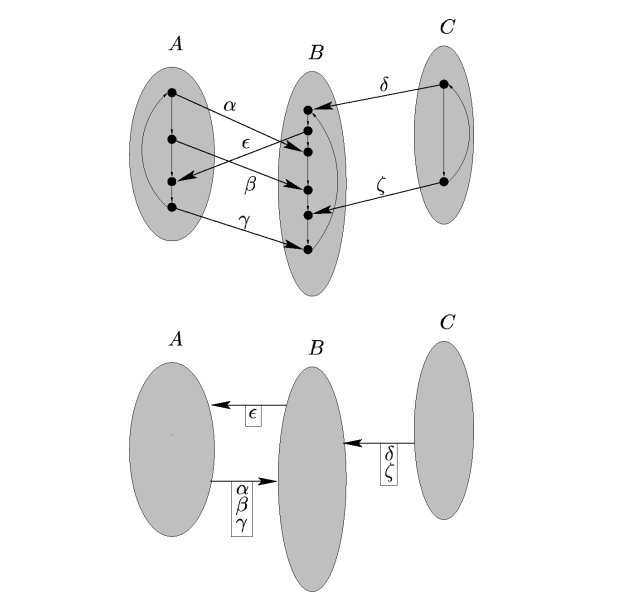
\includegraphics[width = 0.8\textwidth]{graph_models.png}
	\caption[Srovnání stanicového a~rozšířeného modelu.]{Srovnání stanicového a~rozšířeného modelu. Na horním obrázku je rozšířený model. Každý vrchol reprezentuje časovou událost. Pobytové hrany jsou uvnitř stanice; přejezdové hrany mezi stanicemi reprezentují elementární spojení (značena řeckými písmeny). Na dolním obrázku je stanicový model. Každá hrana obsahuje alespoň jedno elementárních spojení. Převzato z~\cite{pyrga2008efficient}.}
	\label{pic:graph_models}
\end{figure}

Zadruhé se jedná o~hrany pobytové. Tyto hrany se vytvoří tak, že se nejprve seřadí všechny vrcholy náležící právě jedné stanici vzestupně dle časového ohodnocení. Poté jsou spojeny pobytovou hranou vždy dva po sobě jdoucí vrcholy. Z~posledního vrcholu této množiny je vedena hrana do prvního vrcholu, která kompletuje smyčku pobytových hran ve stanici. Zdaleka nemusí platit, že jsou propojeny vždy odjezdové a~příjezdové vrcholy stejné jízdy, především tehdy, je-li pobytová doba spoje ve stanici relativně dlouhá. Ohodnocení hrany je možno najít pouhým rozdílem času po sobě jdoucích událostí (konkrétně událost příjezdu a~odjezdu u~přejezdových hran).
\renewcommand{\figureautorefname}{obrázku}
\renewcommand{\subsectionautorefname}{pododdíle}
\subsection{Stanicový model (time-dependent)}
Stanicový model je také digraf, avšak oproti předchozímu modelu obsahuje podstatně méně vrcholů. Každá stanice je totiž reprezentována pouze jedním vrcholem, který je spojen hranou s~vrcholy ostatních stanic právě tehdy, existuje-li mezi stanicemi elementární spojení alespoň jednoho spoje. I~když je spojení více, pořád se jedná jenom o~jednu hranu, která si uchovává informace o~všech časech odjezdu a~příjezdu mezi dvěma stanicemi. 

Z~toho vyplývá, že narozdíl od rozšířeného modelu není ohodnocení hran pevně stanoveno. Časové ohodnocení se totiž přímo odvíjí od toho, v~jaký čas Dijkstrův algoritmus hranu používá, jak je popsáno v~\autoref{casoveZavGrafy}. 

\renewcommand{\subsectionautorefname}{pododdíl}

\subsection{Srovnání modelů}
Rozšířený model vyžaduje mnohem více vrcholů a~je tak paměťově náročnější, zato ale jeho struktura dovoluje jednodušší implementaci algoritmů pro nalezení nejkratší cesty, protože je ohodnocení hran pevně stanoveno. Naopak paměťově méně složitý stanicový model vyžaduje dodatečnou modifikaci algoritmu pro výběr hranového spojení. 

V experimentech nad různě velkými reálnými daty bylo vypozorováno, že stanicový model je časově rychlejší než jeho protějšek, a~to jak u~zjednodušených, tak i~u~realistických úloh \cite{pyrga2008efficient}. Právě tato časová efektivita stanicového modelu je hlavním důvodem, proč je v~implementační části preferován tento model grafu jízdních řádů nad rozšířeným modelem. Jak je však rozvedeno do detailů v~dalším oddíle, pro správné fungování stanicového modelu v~reálném dopravní síti je nutné přistoupit k~několika úpravám, které si vypůjčují prvky rozšířeného modelu. Nicméně primární odlišnost v~přejezdových hranách a~elementárních spojeních zůstává zachována.

\section{Modifikace stanicového modelu}
Následující oddíl detailněji popisuje strukturu základního stanicového modelu. Poté jsou zmíněny realistické požadavky na vyhledávání spojů v~jízdním řádu, jako např. zakomponování přestupních dob do modelu grafu. V~návaznosti jsou navrženy nástavby a~úpravy nutné k~tomu tyto požadavky splnit. Na takto modifikovém stanicovém modelu lze spustit Dijkstrův algoritmus mírně upravený pro časově závislé grafy (TD-Dijkstra).

\subsection{Zákaz předjíždění spojů}
V prvé řadě, aby mohl být Dijkstrův algoritmus použitý pro stanicový model, musí být zajištěno, že se na hraně spoje nemohou předjíždět. Jedná se o~tzv. FIFO\footnote{\textquote{First-In, First-Out} (první dovnitř, první ven)} podmínku o~předjíždění.

\begin{description}
	\item[FIFO podmínka o~předjíždění] Pro spojení \(c\) ze stanice \(A\) do stanice \(B\) platí, že neexistuje jiné spojení \(c^{i}\) mezi stejnými stanicemi, kde \(c^{i}_{\text{odj\_}\tau} \geq c_{\text{odj\_}\tau}\) a~zároveň \(c^{i}_{\text{prij\_}\tau} < c_{\text{prij\_}\tau}\). Tedy \(c\) není předjeto jiným spojem.
\end{description}

Algoritmus standardně kontroluje každou hranu pouze jednou. Pokud by z~nějakého vrcholu \(v\) spoj vyjel první v~pořadí a~přijel do jiného vrcholu \(w\) jako druhý v~pořadí, algoritmus by najednou musel kontrolovat i~další, pozdější spojení na té hraně, protože by mohly ohodnocení \(w\) vylepšit. Proto by byl bez této podmínky výpočet mnohem náročnější.

\subsection{Realistické přestupy}
\label{prestupyTD}
V základním stanicovém modelu je každá stanice reprezentována pouze jedním vrcholem. Ve skutečnosti však tato stanice obsahuje několik různých fyzických stanovišť zastávek, mezi kterými je možno se přemisťovat. Tyto individuální zastávky jsou také zaznamenány v~jízdních řádech. Model musí umožnit pěší přesun mezi stanovišti zastávek. Pro jednoduchost není brán v~potaz pěší přesun mezi zastávkovými stanovišti, které nespadají pod jeden dopravní uzel (stanici), i~když jsou teoreticky v~docházkové vzdálenosti.

Základní verze algoritmu zanedbává přestupní doby, a~tak je možné přijet v~čase \(\tau\) na jednu konkrétní zastávku ve stanici \(A\) spojením \(c\), přestoupit na jiné spojení \(c^i\) (klidně z~jiného stanoviště stanice), kde \(c_{\text{spoj\_id}} \neq c^i_{\text{spoj\_id}}\), a~odjet v~čase \(\tau\). V~realitě však přestup trvá nenulovou dobu a~je nutno tento fakt zakomponovat do modelu. Nabízí se řešení nastavit minimální délku přestupní doby ve stanici při přechodu mezi zastávkami. Pokud je spojení součástí předchozí jízdy (to znamená, že cestující již do vozidla nastoupil v~dřívější stanici), minimální doba přestupu je nulová; v~opačném případě je plošně nastavena jednotná přestupní doba, kterou cestující potřebuje k~provedení přestupu. 

Toto jednoduché řešení je však po řádné kontrole nevyhovující kvůli tomu, jakým způsobem Dijkstrův algoritmus ohodnocuje vrcholy, i~když je respektována FIFO podmínka o~předjíždění.

\begin{figure}[htbp]
	\centering
	\FIFO
	\caption[Selhání stanicového modelu při zavedení realistických přestupů.]{Algoritmus nalezne optimální řešení ve stanicovém modelu pouze v~případě nulové přestupní doby. Je-li přestup delší než dvě minuty, z~\textcolor{BlueViolet}{modrého} spoje, který je využitý mezi \(s\) a~\(a\), nelze přestoupit na \textcolor{RedOrange}{oranžový} spoj, přestože v~počáteční stanici byl teoreticky dosažitelný.}
	\label{fifo}
\end{figure}

Nechť je situace jako \autoref{fifo}, ve které cestující chce jet z~počátku \(s\) do cíle \(t\) v~čase \(\tau = 9\). Nejdřívější spojení, které algoritmus zkontroluje, je z~vrcholu \(s\) do \(a\) na modrém spoji. Cestující tak do \(a\) dorazí v~čase 12. Dle FIFO podmínky není potřeba kontrolovat spojení z~vrcholu \(s\) s~pozdějším odjezdem. Aby se cestující dostal do cílového vrcholu, musí nyní přestoupit na oranžový spoj, protože modrý spoj pokračuje pouze do vrcholu \(b\). Pokud by byla přestupní doba nulová, nebyl by s~přestupem problém. Ale v~situaci, kdy přestup trvá více než dvě minuty, oranžové spojení do cíle není dosažitelné (\(12+3\geq 14\)), a~to i~přesto, že kdyby cestující nastoupil na oranžový spoj hned v~počátku \(s\), cíl by byl dosažen v~čase 17.


\renewcommand{\figureautorefname}{obrázek}
Elegantním řešením, které se inspiruje rozšířeným modelem, je zavedení linkových vrcholů ke stávajícím staničním vrcholům (viz \autoref{pic:tdmodel}) \cite{pyrga2008efficient}. Každý linkový vrchol náleží právě jedné stanici. Ve zjednodušené verzi této úpravy se dá říci, že podle toho kolik linek zastavuje v~dané stanici, tolik linkových vrcholů stanice obsahuje. Linkový a~staniční vrchol je vždy spojen dvěma orientovanými hranami, jedna v~každém směru. Ohodnocení hrany vycházející z~linkového vrcholu je nulové; to znamená, že jakmile je v~algoritmu dosažen jakýkoliv linkový vrchol, je to jako kdyby byl dosažen staniční vrchol. Ohodnocení hrany vycházející ze staničního vrcholu je rovno pevné hodnotě minimální doby přestupu, která modeluje přesun cestujícího mezi stanovišti.

\begin{figure}[htbp]
	\centering
	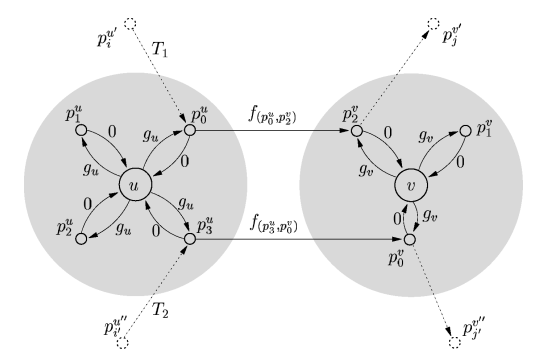
\includegraphics[width=0.8\textwidth]{tdmodel.png}
	\caption[Modifikace stanicového modelu s~reálnými přestupními dobami.]{Modifikace stanicového modelu s~reálnými přestupními dobami. Notace původních autorů: \(u\) je staniční vrchol, \(p_{0}^{u}\) je linkový vrchol, \(g_u\) je doba na přestup. Linka je sled linkových vrcholů. Převzato z~\cite{pyrga2008efficient}.}
	\label{pic:tdmodel}
\end{figure}

Princip je takový, že když cestující pokračuje v~jízdě ve vozidle, ve kterém se aktuálně nachází, nedochází k~přestupu. V~opačném případě se dostane do \textquote{centrálního} vrcholu, odkud může přestoupit na jinou linku. Důležité je, že algoritmus prozkoumá nejdříve jedoucí spojení každé linky a~ne pouze nejdřívější spojení na daném mezizastávkovém úseku.\footnote{Na každé lince zvlášť stále musí platit FIFO podmínka o~předjíždění.} Tento přístup navíc eliminuje potřebu explicitně vzájemně propojovat stanoviště zastávky jedné stanice, protože každý linkový vrchol je automaticky spojen se staničním vrcholem, nehledně na tom, na jakém konkrétním fyzickém stanovišti spoje zastavují. Tudíž je možné mezi linkovými vrcholy, a~v~širším slova smyslu i~stanovišti, volně přecházet. 

\subsection{Trasa místo linky}
Použití linky však také není zcela korektní, protože na běžné dopravní síti často spoje jedné linky obsluhují odlišné sledy stanic během dne nebo týdne. Z~toho důvodu by pak mohla nastat situace, že cestující vystoupí z~jednoho spoje do druhého spoje téže linky, který ale má od daného vrcholu odlišnou trasu. Tento přestup by se počítal, nesprávně, jako nulový. V~praxi k~sice těmto situacím dochází spíše výjimečně, protože spoje jedné linky jezdí v~dostatečně dlouhém intervalu, nicméně při hledání cest bez přestupu by toto zjednodušení vykazovalo nežádané chování (např. by cestující vystoupil z~jednoho spoje linky a~počkal několik minut na další spoj, který zatahuje do depa a~má odlišnou trasu, aniž by se započítal přestup).

Z toho důvodu jsou zavedeny \textit{trasy} a~k~nim příslušné trasové vrcholy namísto původních linkových. Každá trasa je definována jako unikátní sled zastavení, ve kterém se mohou stanice opakovat. K~trase mohou být přiřazeny spoje jedné či více linek a~zároveň spoje jedné linky mohou být přiřazeny k~jedné nebo více trasám. Každý spoj je však přiřazen pouze k~právě jedné trase a~žádná trasa není prázdná.\footnote{Pro jazykovou přehlednost je občas název \textquote{linka} taktéž vnímám jako unikátní sled, i~když to zpravidla není ve skutečnosti pravda.}

\section{Algoritmy pro časově závislé grafy}
Je-li vytvořen model grafu s~časově závislými hranami, je možné pomocí Dijkstrova algoritmu a~jeho úprav nalézt nejkratší cestu v~jízdních řádech. Délka nejkratší cesty je v~těchto grafech značena \(d(s,t,\tau)\), kde \(\tau\) indikuje počáteční čas. 

Ve zbytku tohoto oddílu jsou popsány adaptace některých statických algoritmů zmíněných v~\autoref{ch:algos} pro dynamický stanicový model.

\subsection{Oboustranné vyhledávání}
U statického grafu je oboustranné vyhledávání poměrně snadná záležitost, jenom je potřeba oproti jednostrannému Dijkstrova algoritmu pozměnit podmínku ukončení. Naopak u~časově závislých grafů typu jízdních řádů je na první pohled problematické, že není znám čas příjezdu do cílové stanice, a~tak nelze jednoduše začít zkoumat graf v~opačném směru. Existuje však metoda, jak tento problém částečně vyřešit \cite{NanniciniBiDiA}.

\renewcommand{\figureautorefname}{obrázku}
V dopředném směru je postup časově závislého Dijkstrova algoritmu standardní, tedy že je hledána cesta o~délce $d(s,t,\tau)$. Ve zpětném hledání je obrácený graf převeden do statického grafu, ve kterém je ohodnocení každé hrany minimální cestovní doba ze všech spojení na té hraně a~také je zanedbána přestupní doba. Jakmile se obě vyhledávání střetnou ve vrcholu $v$, končí první fáze algoritmu. Ve druhé fázi je spočtena skutečná délka cesty z~$s$ do $t$ přes $v$ v~dopředném směru s~opravdovým ohodnocením. Toto je horní odhad $\mu$. Obě vyhledávání pokračují do té doby, než se ve zpětné prioritní frontě nachází pouze vrcholy s~minimálním ohodnocením větším než $\mu$. Pak druhá fáze končí. V~poslední fázi je v~dopředném směru vyhledána nejkratší cesta s~tím omezením, že jsou prohledávány pouze vrcholy v~množině vrcholů nalezené zpětným vyhledáváním. Fáze jsou vidět na \autoref{pic:bidijkstra}.
\renewcommand{\figureautorefname}{obrázek}

\begin{figure}[htbp]
	\centering
	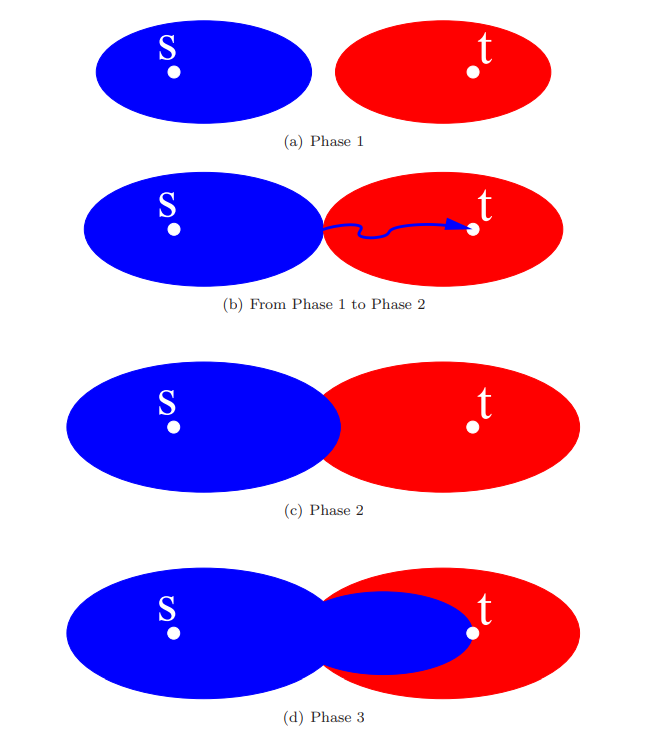
\includegraphics[width = 0.6\textwidth]{bidijkstra.png}
	\caption[Fáze oboustranného Dijkstrova algoritmu v~dynamickém grafu.]{Fáze oboustranného Dijkstrova algoritmu v~dynamickém grafu. Zpětné vyhledávání v~první a~druhé fázi je ve statickém grafu. Převzato z~\cite{NanniciniRoadNetw}.}
	\label{pic:bidijkstra}
\end{figure}

\renewcommand{\sectionautorefname}{oddíle}
\subsection{A* }
V \autoref{staticASTAR} o~A* byly uvedeny některé základní metriky, podle kterých je možné odhadnout vzdálenost vrcholu $v$ do cíle $t$. Pro nalezení nejrychlejší cesty nelze rovnou použít např. Eukleidovskou metriku, jelikož vrcholy jsou ohodnoceny časem (\(t\)), zatímco odhad metriky je vzdálenost (fyzikálně \(s\) pro dráhu). Nabízí se možnost využít fyzikální vztah $t = \frac{s}{v}$. Rychlost \(v\) ale musí být zvolena tak, aby odhady doby jízdy mezi dvěma vrcholy byly přípustné (viz přípustná funkce v~\autoref{staticASTAR}). To však v~multimodálním dopravním systému znamená, že při základní implementaci musí být zvolena \emph{maximální} rychlost prostředku v~daném systému, typicky dálkových vlaků a~autobusů. Jelikož mnoho vozidel však dosahuje mnohem nižších průměrných rychlostí (např. městské autobusy), je tak dolní odhad velmi konzervativní.

\renewcommand{\subsectionautorefname}{pododdíle}
V případě zjednodušené úlohy, ve které je zakázáno přestupovat mezi jednotlivými druhy prostředků, je možné dolní odhady mírně upřesnit. Pokud se vrchol $v$ nachází $x$ metrů od cíle přímou čarou (dle Eukleidovské metriky), bude doba dolního odhadu pro jízdu pražskými tramvajemi téměř dvojnásobná než u~metra \cite{DPPvDatech}. Umožnění přestupů mezi prostředky je však běžná a~základní vlastnost systémů VHD, proto je nutné hledat další alternativy, jako například landmarky popsány v~\autoref{staticLANDMARKS}.
\renewcommand{\subsectionautorefname}{pododdíl}

\subsection{Landmarky (ALT)}
Tak jako se na silniční síti počítá nejkratší cesta mezi landmarkem a~všemi ostatními vrcholy a~opačně, v~časově závislém grafu se jedná o~nejrychlejší cestu. Existují dva způsoby výpočtu nejrychlejší cesty. První, méně přesná metoda určuje nejrychlejší cestu v~grafu za předpokladu, že každá hrana je ohodnocena nejkratší dobou přejezdu, jaká se v~jízdním řádu vyskytuje, aby nedošlo k~přecenění vzdálenosti. Přestože se doby přejezdu mezi jednotlivými spojeními zpravidla příliš neliší, tato metoda nezohledňuje čas strávený čekáním na přípoj \cite{dellingLandmarkRouting}.

Druhá metoda je pracuje s~tím, že se nejrychlejší cesta různí podle toho, v~jaký den a~hodinu je potřeba se přemístit. Výpočet cesty z~$v$ k~landmarku (a~obráceně) je v~pre-processingu proveden během jednoho dne např. ve dvouhodinových intervalech. V~této fázi je potřeba použít tzv.~\textquote{profilové hledání}, aby se našla doba nejrychlejší cesty s~časem odjezdu kdekoli v~daném intervalu. Poté při ohodnocování vrcholů algoritmus pracuje s~těmi hodnotami odhadované cestovní doby, podle toho, v~jakém časovém intervalu byl vrchol (opětovně) dosažen.

\renewcommand{\figureautorefname}{obrázek}
U obou technik ve fázi pre-processingu dochází k~tomu, že je ve statickém grafu vypočten strom nejkratších cest z~každého landmarku do ostatních vrcholů. Rovněž musí být zjištena i~vzdálenost od každého vrcholu do každého landmarku, což lze efektivně učinit tak, že se vypočítá strom nejkratších cest z~landmarků v~obráceném grafu \(G\). 

\subsection{Contraction hierarchies}
Při zkracování vrcholu a~vytvoření zkratky ve statickém grafu docházelo ke sjednocení vstupní a~výstupní hrany z~daného vrcholu. U~časově závislých grafů je nutné zavést sjednocení jednotlivých spojení, která mohou náležet různým spojům. Např. mezi vrcholy $u$ a~$w$, když je $v$ zkracován, je vytvořena nová kombinace spojení pro každé spojení na hraně (u,v) s~každým spojením na hraně (v,w). Není nutné zavádět spojení pro dominovaná spojení anebo pokud existuje alternativní rychlejší spojení neprocházející $v$, tzv.~\textquote{witness} cesta \cite{wirthCHDiploma}.

Efektivní nalezení těchto alternativní cest je stěžejní pro rychlost algoritmu, jelikož to zabírá podstatnou část pre-processingu. Je nutné projít všechna spojení $c$, která mají být zrušena nebo nahrazena, a~zjistit, jestli existuje alternativní sled spojení, který odjíždí z~$u$ později než $c_{\text{odj\_}\tau}$ a~přijede do $v$ dříve než $c_{\text{prij\_}\tau}$. Poměrně složité metody jsou popsány v~\cite{BatzTDCH} nebo \cite{wirthCHDiploma}.

\section{Algoritmy bez grafové struktury}
Pro modelování problému nejkratší cesty v~jízdních řádech byly zkonstruovány i~algoritmy, které nevyžadují strukturu grafu, nejsou bázované na Dijkstrově algoritmu a~nevyužívají prioritní frontu. Právě ta poslední zmiňovaná vlastnost slibuje rychlejší vyhledávání cesty, protože manipulace prioritní fronty je vcelku časově náročná operace \cite{CMUBinHeaps}.

\subsection{RAPTOR}
Prvním z~nich je RAPTOR (Round bAsed Public Transit Optimized Router), se kterým přišel tým autorů Delling et al. \cite{dellingRAPTOR}. RAPTOR byl navržen pro získaní všech pareto-optimálních cest a~ne pouze cesty s~nejdřívějším příjezdem (více v~\autoref{sec:kriteriaOptCesty}). Algoritmus je založený na jednotlivých kolech (rounds), ve kterých je traverzována každá linka (popř. trasa) maximálně jednou. Pořadí kola indikuje dovolený počet přestupů: v~prvním kole není dovolený žádný přestup, v~druhém jeden, atd.

V úvodní fázi prvního kola jsou navštívené pouze stanice, které jsou dosažitelné z~počátku, aniž by byla potřeba přestupovat mezi linkami. Je vybírán vždy spoj, jehož čas odjezdu je nejmenší a~větší než \(\tau\). V~další fázi jsou dovoleny pěší přesuny mezi stanovišti zastávek dosažených stanic. Na konci každého kola je zaznamenáno časové ohodnocení navštívených stanic. 

V druhém kole je traverzována každá linka -- která je dosažitelná alespoň z~jedné stanice navštívené v~předchozím kole -- od první stanice, ve které je na ni možno nastoupit. Opět jsou zjištěny přestupy mezi stanovišti zastávek a~přidáno ohodnocení. Takto se postupuje do té doby, dokud není dosaženo omezení počtu kol anebo v~předchozím kole nedošlo k~žádnému zlepšení ohodnocení. Seznam pareto-optimálních cest je pak extrahován z~ohodnocení cílové stanice.

Výše byl v~krátkosti popsán pouze základní model; v~\cite{dellingRAPTOR} je rozebráno několik optimalizací a~alternativních modelů jako McRAPTOR nebo rRAPTORr.

\subsection{CSA}
\label{CSAtheory}
Další model se nazývá Connection Scan Algorithm, který byl představen Dibbeltem et al. \cite{dibbelt2017CSA}. Základní idea je taková, že pokud existuje seznam všech elementárních spojení v~daném jízdním řádu seřazených dle času odjezdu, je možné seznam lineárně procházet (\textquote{skenovat}) a~rozhodnout se, jestli dané spojení je dosažitelné z~aktuálního vrcholu \(v\) a~času $\tau$.

V~seznamu $S$ jsou uchovávány nejdřívější příjezdy do stanice. Na začátku algoritmu jsou nastaveny na nekonečno, podobně jako u~standardního Dijkstrova algoritmu.

CSA začíná procházet všechna spojení $c$, která odjíždí z~výchozí stanice $c_{\text{odj\_st}}$ nejdříve v~$\tau_0$, tedy musí platit $c_{\text{odj\_}\tau} \geq \tau_0$. Spojení $c$ je označeno jako dosažitelné právě tehdy, pokud platí alespoň jedna podmínka:

\begin{enumerate}[label = \normalfont\itembox{\roman{enumi})}]
	\item pro některé z~předchozích dosažených spojení $c^i$ platí, že $c^i_{\text{spoj\_id}} = c_{\text{spoj\_id}},$
	\item $c_{\text{odj\_}\tau} \geq S[c_{\text{odj\_st}}]$.
\end{enumerate}

Jinými slovy buďto jízda již byla dosažena v~minulosti (a~tak je zaručeně dosažitelná i~nyní) anebo je možné stanici dosáhnout jiným spojem dříve, než je čas odjezdu $c$ ze stanice (splnění druhé podmínky neimplikuje splnění té první v~případě realistických přestupů, viz níže). Pokud je nové ohodnocení $c_{\text{prij\_}\tau} < S[c_\text{{prij\_st}}]$, je ohodnocení v~příjezdové stanici upraveno.

Podobně jako u~platí u~RAPTORa, oficiální jízdní řády často obsahují přímo specifické zastávky (stanoviště) a~ne pouze stanice, a~tak je nutné zajistit přemístění mezi nimi v~rámci jedné stanice. Tyto cesty se obvykle nazývají \textquote{footpaths} nebo česky \textit{pěšiny}. Tudíž pokaždé, když spojení přijede do stanice, musí být vypočteno nové ohodnocení dosažitelných zastávek pomocí pěšin. Pěšiny jsou ohodnoceny přestupní dobou.

Speciální případ pěšiny je smyčka, která vychází i~končí ve stejné zastávce. Bez této smyčky by nebylo možné na té samé zastávce vystoupit z~jednoho spoje a~zároveň nastoupit do jiného spoje, protože k~ohodnocení zastávek dochází až ve fázi prozkoumávání pěšin. Kdyby tam smyčka nebyla, algoritmus by si nepamatoval, že už zastávku v~minulosti dosáhl. Obvykle jsou i~tyto smyčku ohodnoceny přestupní dobou, i~když menší než u~ostatních pěšin. Výjimka je u~cílové stanice, kde tato smyčka trvá nulovou dobu, protože cestující již je v~cíli (analogicky ke stanicovému modelu, kde je nulový přestup u~výchozí stanice).

Protože existují smyčky s~nenulovou přestupní dobou \(\delta\), je zapotřebí zachovat první podmínku dosažitelnosti spojení: spojení je dosažitelné, když jiné spojení daného spoje již bylo dosaženo dříve. Pokud cestující využije spojení \(c_i\), které na zastávku přijede v~čase \(\tau\) dle jízdního řádu a~poté následující spojení \(c_{i+1}\) z~něj v~ten čas odjede, zastávka bude ohodnocena \(\tau + \delta\). Druhá podmínka dosažitelnosti u~\(c_{i+1}\) zřejmě není splněna, ale ta první ano, takže spojení může být využito.

Algoritmus končí ve chvíli, když je ohodnocení cílové stanice menší nebo rovno času odjezdu aktuálně skenovaného spojení. V~tuto chvíli už žádné spojení nemůže zlepšit ohodnocení cílové stanice, protože čas příjezdu spojení je vždy větší než jeho čas odjezdu.

Způsob nalezení cesty je rozebrán podrobně v~\autoref{csaImplementace}, kde je popsána implementace CSA.

\section{Kritéria optimality cesty a~řešené úlohy}
\label{sec:kriteriaOptCesty}
Dijkstrův algoritmus je schopen řešit úlohu nalezení nejkratší cesty nejen z~jednoho počátku do jednoho cíle, ale i~z~jednoho počátku do několika (nebo všech) ostatních vrcholů. Z~praktických důvodů jsou však algoritmy jízdních řádů primárně zaměřené na nalezení optimální cesty mezi dvěma vrcholy, nicméně speciální algoritmy pro řešení alternativních problémů také existují \cite{geisberger2010TDOneToAll}.

I když se jedná o~nalezení cesty z~jednoho vrcholu do druhého, stále existují různá kritéria, podle kterých se optimalita cesty dá hodnotit. U~klasických statických grafů se volí jako kritérium nejkratší cesta, tudíž i~zde by se nabízelo volit nejkratší jízdní dobu. Ovšem kvůli tomu, jakým způsobem Dijkstrův algoritmus ohodnocuje vrcholy, je nutné kritérium zaměnit za nejdřívější příjezd do cíle od výchozího času. Častečným řešením problému nejrychlejší cesty je zavedení profilových hledání. Další důležitým kritériem je počet přestupů, především v~kombinaci s~nejdřívějším příjezdem. 

Níže zmíněné úlohy jsou v~literatuře standardem, ale jejich definice jsou částečně inspirovány zněním v~\cite{dibbelt2017CSA,pyrga2008efficient}. 

\begin{description}
	\item[Úloha nejdřívějšího příjezdu] Je-li dána počáteční stanice $s$, cílová stanice $t$ a~výchozí čas $\tau_0$, řešením úlohy je nejdřívější čas příjezdu do $t$ s~odjezdem z~$s$ v~$\tau_0$ nebo později. 

	\item[Úloha profilových nejdřívějších příjezdů] Je-li dána počáteční stanice $s$, cílová stanice $t$ a~interval [$\tau_0, \tau_1$], řešením úlohy je nalezení nejdřívějšího času příjezdu pro každý čas odjezdu $\tau \in [\tau_0, \tau_1]$. 
	
	Profilové nejdřívější příjezdy jsou užitečné proto, že cestující má vesměs flexibilitu při výběru času odjezdu a~nejdřívější příjezd není to nejpodstatnější. Díky tomu, že počet odjezdů spojů ze stanice v~ohraničeném časovém intervalu je v~jízdních řádech veřejné hromadné dopravy konečný, není potřeba počítat nejdřívější příjezd pro všechny časy (např. pro každou sekundu). Je dostačující rozdělit původní interval do několika menších podintervalů, z~nichž každý obsahuje pouze jeden odjezd spoje ze stanice.
	
	\renewcommand{\tableautorefname}{tabulku}
	V~praxi to znamená, že algoritmus spočítá nejdřívější příjezd pro každý reálný čas odjezdu spoje ze stanice v~původním intervalu. Cestujícímu se pak mohou nabídnout všechny nedominované nejrychlejší cesty anebo pouze jediná cesta, která je z~celého intervalu nejrychlejší. Nematematicky řečeno se dominovanou cestou v~tomto kontextu myslí taková cesta \(P_d\), pro kterou existuje jiná cesta \(P_i\), která je za všech okolností výhodnější. To nastane tehdy, když je u~\(P_i\) čas odjezdu později a~čas příjezdu dříve než u~\(P_d\) (u~jedné události se časy mohou i~rovnat). Pro příklad viz \autoref{tab:profiledomi}.
		
	\newcolumntype{M}[1]{>{\centering\arraybackslash}m{#1cm}}
	
	\begin{table}[h]

		\centering
		\begin{tabular}{M{1.7}M{1.7}M{1.7}M{1.5}M{2.5}}
			\toprule
			\textbf{Č. cesty} & \textbf{Čas odjezdu} & \textbf{Čas příjezdu} & \textbf{Jízdní doba} & \textbf{Cesta je dominovaná} \\
			\midrule
			1 & 10:10 & 10:45 & 35~min & Ano \\
			2 & 10:15 & 10:45 & 30~min & Ne \\
			3 & 10:15 & 10:50 & 35~min & Ano \\
			4 & 10:20 & 11:00 & 40~min & Ne \\
			\bottomrule
		\end{tabular}
		\caption[Soubor profilových cest a~jejich vzájemné dominance.]{Soubor profilových cest a~jejich vzájemné dominance. Zde cesta č.~2 dominuje cestu č.~1 -- protože čas odjezdu je u~č.~2 později a~zároveň čas příjezdu \emph{není} později než u~č.~1 -- i~č.~3, protože u~č.~2 je čas příjezdu dříve a~zároveň čas odjezdu \emph{není} dříve. Cesta č.~4 není dominovaná, přestože její jízdní doba je o~5 minut delší než u~cesty č.~3; čas odjezdu i~příjezdu je totiž u~ní později.}
		\label{tab:profiledomi}
	\end{table}
\end{description}

	V dopravních sítích není rychlost jediným důležitým kritériem. Rozhodujícím faktorem je totiž i~počet přestupů, a~to do té míry, že cestující je ochoten strávit delší čas na cestě, pokud si ušetří alespoň jeden přestup.\footnote{Empiricky bylo zjištěno, že jeden přestup se v~městské dopravě projeví u~preferencí cestujících jako 5 minutová penalizace oproti cestě s~jedním přestupem méně \cite{heimerl1988german}.} Protože však úloha minimálních přestupů je sama o~sobě nezajímavá (všechny nepřestupní hrany jsou ohodnoceny 0), je vhodné zavést kombinované úlohy.
\begin{description}
	\item[Úloha nejdřívějšího příjezdu s~minimalizací počtu přestupů] \hskip 0.8em Je-li\linebreak dána~počáteční stanice $s$, cílová stanice $t$ a~výchozí čas $\tau_0$, řešením úlohy je cesta s~nejdřívějším časem příjezdu do $t$ s~odjezdem z~$s$ v~$\tau_0$ nebo později. Pokud takových cest je více, je zvolena cesta s~menším počtem přestupů $T$; v~případě rovnosti $T$ je volba cesty náhodná. 

\end{description}
Ačkoliv tato úloha činí výběr cesty rozumnějším, stále existují situace, ve kterých existují dvě alternativní cesty, z~nichž jedna je o~minutu delší než druhá, ale obsahuje o~alespoň jeden přestup méně. Řešením je nabídnout cestujícímu množinu všech pareto-optimálních cest. 

\begin{description}
	\item[Úloha nalezení všech pareto-optimálních cest] Je-li dána počáteční stanice $s$, cílová stanice $t$ a~výchozí čas $\tau_0$, řešením úlohy je množina cest, z~nichž žádná není dominovaná.
	
	Pareto-optimální cesta je taková cesta, která není jinou cestou dominována. Dominance je zde chápána v~odlišném slova smyslu než u~profilových cest, u~kterých záleželo na čase odjezdu a~příjezdu. Zde jsou kritéria pareto-optimalitní cesty nejdřívější příjezd a~počet přestupů, ale kritérií může být obecně více.

	\begin{description}
		\item[Dominovaná cesta] Cestě $P_d$ z~počáteční stanice $s$ do cílová stanice $t$ v~čase $\tau_0$ je možno přiřadit atributy s~hodnotami. U~všech atributů je kritérium minimalizační. Cesta $P_d$ je dominovaná právě tehdy, když existuje jiná $P_i$ z~$s$ do $t$ splňující následující podmínky:
		\begin{enumerate}[label = \normalfont\itembox{\roman{enumi})}]
			\item pro každý z~atributů $P_d$ platí, že jeho hodnota je nejméně tak velká jako hodnota u~$P_i$ a
			\item alespoň jedna hodnota atributu $P_i$ je striktně nižší než hodnota u~$P_d$.  
		\end{enumerate}
	\end{description}
		
		To u~cesty s~atributy nejdřívějšího příjezdu $\tau_0$ a~počtu přestupů $T$ znamená, že cesta $P_d$ je dominována, když je možné se alternativní cestou $P_i$ dostat do cíle dříve a~se stejným nebo menším počtem přestupů (popř. má $P_i$ stejný čas příjezdu, ale má méně přestupů). Všechny nedominované cesty jsou pro cestujícího atraktivní (resp. každý cestující si zvolí cestu dle svých preferencí). Nedominované cesty tvoří pareto-optimální množinu cest. Konkrétní příklad je v~\autoref{tab:pareto-example}.

	\begin{table}[h]
		\centering
		\begin{tabular}{cccc}
			\toprule
			\textbf{Č. cesty} & \textbf{Čas příjezdu} & \textbf{Počet přestupů} & \textbf{Pareto-optimální} \\
			\midrule
			1 & 11:55 & 3  & Ano \\
			2 & 12:00 & 2  & Ano \\
			3 & 12:10 & 1  & Ano \\
			4 & 12:05 & 2  & Ne  \\
			\bottomrule
		\end{tabular}
		\caption[Příklad pareto-optimálních cest]{Soubor tří pareto-optimálních cest (1, 2 a~3), a~jedné cesty (4), která je dominovaná jinou cestou. Cesta č.~1 má nejdřívější čas příjezdu, avšak se třemi přestupy. Cesta č.~2 má čas příjezdu o~pět minut později, ale protože vyžaduje o~jeden přestup méně, není vůči předchozí cestě dominovaná. Podobně je na tom i~cesta č. 3. Avšak cesta č.~4 má o~pět minut pozdější příjezd než cesta č.~2 a~vyžaduje stejný počet přestupů, proto je cesta č.~4 suboptimální.}
		\label{tab:pareto-example}
	\end{table}
\end{description}

\part{Praktická aplikace}
\chapter{Implementace}
\label{implementace}
\renewcommand{\sectionautorefname}{oddíl}
V této kapitole je podrobně popsáno, jakým způsobem jsou modely a~algoritmy implementovány v~programovacím jazyce Python, včetně základního grafického uživatelského rozhraní vyhledávače spojů. Veškeré potřebné soubory k spuštění algoritmů jsou dostupné v~přiložených materiálech k této práci. Struktura a~popis souborů je v~příloze~\ref{appendix_main}, \autoref{appendix_org}.
\renewcommand{\sectionautorefname}{oddíle}

V úvodu kapitoly je zběžně představen dopravní systém Pražská integrovaná doprava (PID) a~formát dat GTFS, pomocí nějž PID zpřístupňuje veškeré informace o~jízdních řádech. Nakonec je zrealizován modifikovaný stanicový model, který kromě Dijkstrova algoritmu využívá A* s~Eukleidovskou metrikou a~landmarků (ALT), a~také negrafový algoritmus CSA. Pomocí těchto algoritmů je pak možné prakticky vyřešit úlohy, které byly představeny na konci předešlé kapitoly.

\section{Otevřená data PID}
\label{opendata}
Pražská integrovaná doprava (PID) je integrovaný dopravní systém na území Prahy a~Středočeského kraje \cite{PIDoSystemu}. Zahrnuje metro, tramvaje, vlaky, městské i~příměstské autobusy, lanovou dráhu a~přívozy. Za správné fungování zodpovídají dva organizátoři, Regionální organizátor pražské integrované dopravy, p. o. (ROPID) a~Integrovaná doprava Středočeského kraje (IDSK). Cílem PID je vytvořit kompatibilní dopravní obsluhu území se sjednocenými přepravními a~tarifními podmínkami a~zajistit koordinaci spojů v~jízdních řádech. 

Území, které pokrývá PID veřejnou hromadnou obsluhou, slouží jako podklad k~nadcházejícím algoritmům, protože nejrychlejší cesty jsou hledány právě v~jízdních řádech PID. Oblast Prahy a~okolí byla zvolena primárně proto, že PID volně zpřístupňuje různé datové sady přímo na internetové stránce v~rámci projektu otevřených dat \cite{PIDOPENDATA}. Pro tuto práci je podstatná pouze sada s~jízdními řády ve formátu GTFS a~podrobný seznam zastávek, nicméně na oficiální stránce lze získat přístup i~k~aktuální poloze vozů či seznamu prodejních míst PID.

\section{GTFS: obecný úvod}
Nejběžnějším formátem pro ukládání dat typu jízdních řádů je General Transit Feed Specification (GTFS) \cite{gtfsStarted}. Jedná se standardizovaný a~celosvětově využívaný formát, který umožňuje konzistentní manipulaci dat napříč různými regiony a~dopravními systémy. Jelikož jsou data otevřená a~transparentní, jsou běžně využívána softwarovými aplikacemi pro plánování a~vizualizaci tras nebo zobrazení informací v~reálném čase.

GTFS se skládá ze dvou hlavních částí: GTFS Schedule (nebo též GTFS Static) a~GTFS Realtime. GTFS Realtime využívá dynamická data a~zobrazuje cestujícím aktuální informace o~tom, jaké stanice a~linky jsou aktuálně v~provozu, a~také informuje o~poloze a~plánovaném nebo aktuálním zpoždění spojů \cite{gtfsDocumentation}. Aktualizace dat probíhá každých pár sekund.

U GTFS Schedule k~aktualizaci dat naopak dochází periodicky, typicky denně (jako u~PID) nebo týdně. Tato data obsahují mimo jiné informace o~zastávkách, linkách či jednotlivých spojích, a~to obvykle na 14 dní dopředu; proto některé informace o~zastávách mohou chybět, pokud je např. zastávka dočasně mimo provoz. Tato práce využívá pouze statická data GTFS Schedule, jejichž strukturu popisuje následující oddíl detailněji.

\subsection{GTFS Schedule}
Každá datová sada z~GTFS Schedule (dále jen GTFS) je složena z~několika CSV souborů s~příponou názvu souboru \texttt{.txt}. Těchto souborů může být několik desítek, ale pouze několik málo z~nich je povinných \cite{gtfsDocumentation}. Tyto povinné soubory jsou zároveň ty, které tvoří kostru celé datové sady a~poskytují nejdůležitější informace. Jedná se o~soubory: \texttt{agency, stops, routes, trips, stop\_times} a~\texttt{calendar}.

\begin{itemize}
    \item{\texttt{agency} –  Obsahuje informace o~dopravcích. V~případě dat PID je však uveden pouze dopravce \textquote{PID} kvůli jednotnosti tarifu. Konkrétní smluvní dopravci jsou uvedeni v~jiném souboru.}
    \item {\texttt{stops} – Obsahuje popis aktuálně provozovaných zastávek a~stanic.}
    \item {\texttt{routes} – Obsahuje informace o~aktuálně provozovaných linkách.}
    \item {\texttt{trips} – Obsahuje soupis spojů, které jsou přiřazeny k~linkám.}
    \item {\texttt{stop\_times} – Obsahuje informace o~čase odjezdu a~příjezdu spoje na zastávku.}\footnote{Spojení lze složit z~páru dvou po sobě jdoucích záznamů u~jednoho spoje. Jedná se o~složení stanice a~času odjezdu v~prvním záznamu a~stanice a~času příjezdu v~druhém záznamu.}
    \item {\texttt{calendar} – Udává platnost jízdních řádů. Každý spoj se odkazuje na právě jeden záznam, který zahrnuje rozmezí dnů, kdy jízdní řád platí, a~zároveň vymezuje dny v~týdnu (např. víkend).}
\end{itemize}
    
\section{Načtení dat a~tvorba zastávek}
Sadu GTFS dat jízdních řádu od PID je potřeba stáhnout do lokálního nebo cloudového úložiště. Z~něj jsou pak data načtena při spuštění kódu. Ve fázi pre-processingu jsou některé textové soubory zkombinovány a~je vytvořena tabulka jízdních řádu (například záznamy ze \texttt{stop\_times} jsou spárovány s~\texttt{trips} a~\texttt{routes}, aby byly vytvořeny vrcholy pro jednotlivé trasy a~získány uživatelsky přívětivé názvy linek). 

Dále je potřeba získat seznam všech zastávek. Bohužel základní GTFS soubor \texttt{stops} je nedostačující, protože se v~něm objevují zastávky se stejnými jmény, aniž by patřily pod stejnou stanici (\textquote{Všechlapy} na Benešovsku a~\textquote{Všechlapy} na Nymbursku) či navíc označují zastávku různých dopravních prostředků. Z~toho důvodu je nutné stáhnout i~soubor \texttt{Seznam zastávek.json}, který obsahuje unikátní názvy zastávek [Všechlapy (BN), Všechlapy (NB); Chýně, Chýně (vlak)]. U~takto upraveného seznamu zastávek jsou stále zachovány rozdílné názvy zastávek patřící pod jednu stanici neboli dopravní uzel (např. dopravní uzel \textit{Dejvická} zahrnuje jak stanici metra \textit{Dejvická}, tak zastávky autobusů a~tramvají \textit{Vítězné náměstí}). 

Protože načítání textových souborů a~složitá manipulace nad nimi je časově náročná, jakmile jsou základní tabulky jednou načteny, jejich parametry jsou rovnou uloženy v~tomto stavu a~při dalším spuštění algoritmu již nedochází k~opakované rekonstrukci.\footnote{Konkrétně je pro ukládání a~získávání dat použita knihovna \texttt{joblib} a~metody \texttt{joblib.save} a~\texttt{joblib.load}.}

\section{Vytvoření grafu}
\subsection{Vytvoření vrcholů}
Jeden záznam spojení v~tabulce jízdních řádů mimo jiné obsahuje zastávku odjezdu a~příjezdu. Toto je obvykle značeno kódem ve tvaru \texttt{U321Z6P} (\textit{Dejvická}, stanoviště 6). Číslo před \texttt{Z} identifikuje stanici, číslo po \texttt{Z} stanoviště zastávky. Staniční vrchol je interně značen ve stylu \texttt{U321} a~reprezentuje abstraktní střed, ve kterém cestující začíná a~končí svou cestu (vždy v~různých stanicích).

Model s~realistickými přestupy navíc vyžaduje linkové vrcholy, kterých je zpravidla větší množství. Postup jejich vytvoření je následující: \begin{enumerate}[label = \normalfont\itembox{\roman{enumi})}]
	\item vytvoří se slovník, který obsahuje všechny unikátní sledy zastávek v~jízdním řádu jako klíče
	\item každému sledu je přiřazeno unikátní číslo
	\item každé ID spoje je napárováno s~unikátním číslem pomocí sledu zastávek
\end{enumerate}

\subsection{Úprava dne a~času odjezdu a~příjezdu}
Po předchozím kroku je nyní možné z~tabulky jízdních řádů vytvořit hrany grafu. Jízdní řády jsou ale již ze své podstaty založeny na periodicitě, a~tedy mnoho informací je v~nich duplikovaných. Pokud spoj jede každý pracovní den vždy ve stejný čas, jedná se o~pět záznamů, které si jsou velmi podobné. Jednodušší je tak v~grafu vytvořit pouze jeden záznam spoje obsahující seznam zastávek s~časy odjezdu a~příjezdu a~přiložit k~němu datovou strukturu dne platnosti. Den platnosti v~sobě uchovává informace podobné GTFS souboru \texttt{calendar}, tedy rozmezí dnů a~dny v~týdnu, kdy spoj jede (např. od 3. 7. 2025 do 31. 7. 2025, každý pracovní den). Tímto je zajištěna kompaktnost informací u~každé hrany.

Jednou komplikací je zvláštnost GTFS záznamů v~souboru \texttt{stop\_times}: spoje v~brzkých ranních hodinách jsou obvykle značeny časem, který překračuje standardních 24 hodin. Proto spoj může klidně zahájit jízdu ve 24:30 a~ukončit ji ve \textquote{26:01}. Typicky se jedná o~noční linky, ale není to podmínkou. Výhodou je, že je zachována časová platnost z~předchozího dne, a~tak se všechny odjezdy spoje, který zahajuje jízdu v~neděli v~noci a~ukončuje ji v~pondělí brzy ráno, vztahují na jízdní řád platný v~neděli, resp. o~víkendu.

Každopádně tuto časovou abnormalitu je potřeba ošetřit. Nabízí se řešení převést odjezdy a~příjezdy po 24:00 na další den (24:30 → 00:30 +1 den). Toto řešení je určitě schůdné, jenže Dijkstrův algoritmus ohodnocuje vrcholy v~sekundách, a~tak je výhodnější, že implicitně je čas 24:30 větší než 23:50, zatímco 0:30 není. Při průchodu algoritmem by pak nejdřívější čas odjezdu ze zastávky bylo modulo 24 h aktuálního ohodnocení vrcholu. Další komplikací je, že algoritmus by automaticky předpokládal, že spojení s~odjezdem např. v~pondělí 02:30 musí mít i~den platnosti v~pondělí; to není vždy pravda, protože to je pravděpodobně noční spoj s~dnem platnosti v~neděli. Proto by tak musely být spoje překračující 24 hodin speciálně označeny. 

Existuje alternativní řešení, které je jednodušší na pochopení a~dochází k~menší úpravě samotného algoritmu, ale za cenu většího nároku na paměť. Implementované řešení totiž duplikuje spojení, která mají odjezd nebo příjezd po 24:00, ale odečítá jim 24 hodin z~času odjezdu a~příjezdu. Díky tomu v~čase odjezdu v~01:15 budou prohledávány i~spoje, které jedou po 25:00. Pro datovou konzistenci mají tato nově vytvořená spojení označení, že jejich den platnosti je posunut o~jeden den dopředu vůči původnímu dnu odjezdu (např. že v~pondělí ráno může být využit pouze noční spoj z~neděle a~nikoliv z~pondělí).

Analogicky když je výchozí čas nastaven na 23:59, může nastat problém, že brzký ranní spoj denní linky z~následujícího dne nebude moci být použit, protože není dostupný. Proto ranní spoje do 06:00 jsou duplikovány dopředu o~24 hodin a~jsou pak označeny jako patřící předchozímu dni platnosti (tj.~že i~když bylo vyhledávání cesty zahájeno v~neděli v~noci, duplikované denní jízdy s~dnem platnosti pouze v~neděli nesmí být využity). 


\subsection{Vytvoření hran}
Nyní je možné iterovat předpřipravenou tabulkou jízdních řádů, která je seřazena dle identifikačního čísla spoje a~také pořadí navštívených zastávek. Každý záznam je jedno elementární spojení. Všechna elementární spojení mezi totožným párem linkových vrcholů jsou obsaženy v~ohodnocení jedné orientované hrany, tzn.~že hrana obsahuje seřazený seznam těchto elementárních spojení dle času odjezdu. Zároveň z~každého linkového vrcholu vede orientovaná hrana s~nulovým ohodnocením do příslušného staničního vrcholu; opačným směrem pak vede hrana s~ohodnocením odpovídajícím minimální době na přestup (běžně ponechána na 180~s). Některé spoje mohou zastavovat na dvou po sobě jdoucích zastávkách, jež obě patří pod jednu stanici. Toto však neovlivňuje správnost algoritmu.

Je nutné zmínit, že vytvoření těchto hran není instantní, ale trvá kolem 4 až 5 sekund. Tato operace by běžně byla provedena pouze jednou a~pak uložena na serveru, nicméně při \textquote{domácím} spuštění programu ji je nutno pokaždé opakovat. Jakmile je však program spuštěn, je možné provést libovolné množství vyhledávání nejrychlejších cest, protože hrany jsou již načteny.

\section{Základní Dijkstrův algoritmus}
V této fázi je již vše připraveno pro spuštění základního algoritmu pro vyřešení úlohy nejdřívějšího příjezdu. Na ni pak další úlohy úzce navazují. Kvůli odlišení se tento dynamický Dijkstrův algoritmus, který je aplikován ve stanicovém modelu, bude nadále nazývat TD-Dijkstra (od \textquote{time-dependent Dijkstra}).

\subsection{Úloha nejdřívějšího příjezdu}
Uživatel si zvolí počáteční stanici $s$, cílovou stanici $t$, čas odjezdu $\tau_0$ a~den odjezdu $D$. Počátek je vždy ve staničním vrcholu (jak bylo vysvětleno výše, u~některých názvů zastávek je počáteční vrchol identický, jako u~stanice \textit{Dejvická} a~zastávky \textit{Vítězné náměstí}). Všechny hrany z~výchozí stanice mají za běhu změněno ohodnocení na nulu, protože na začátku nedochází k~žádnému přestupu.

Prioritní fronta je implementována pomocí knihovny \texttt{heapq}. Když algoritmus vybere z~prioritní fronty linkový vrchol stanice v~čase $\tau$ a~dni \(D\), jsou skenováni ještě neprobraní sousedi. To v~praxi znamená zkoumání \textquote{přesunu} do staničního vrcholu anebo zahájení jízdy či její pokračování. Je-li sousední vrchol také linkový vrchol, je vybráno spojení mezi nimi, kde čas odjezdu $c_\text{odj\_}\tau$ je nejnižší a~$c_\text{odj\_}\tau \geq \tau$ a~zároveň $D$ je v~intervalu dne platnosti daného spoje. Efektivní řešení nalezení spojení je pomocí binárního vyhledávání, které nejprve nalezne první spojení s~vyhovujícím časem odjezdu, a~pak postupně probírá další spojení, dokud není nalezeno první s~validním dnem platnosti.

Následně je ohodnocení vybraného sousedního vrcholu sníženo a~předcházející vrchol $P(v)$ je aktualizován, je-li čas příjezdu nového spojení nižší než předchozí ohodnocení, jinak jsou hodnoty ponechány stejné. Jakmile je z~prioritní fronty vybrán cílový vrchol $t$, vyhledání cesty s~nejdřívějším příjezdem je ukončeno. Pomocí předchůdců $P(v)$ je možné zkonstruovat přesné pořadí vrcholů této cesty.

Zajímavější než nejdřívější příjezd je doba jízdy, která však v~této úloze není TD-Dijkstrou nutně minimalizována; lze ji získat jako rozdíl příjezdu do cílové stanice a~odjezdu z~té počáteční $c^k_{\text{prij\_}\tau} - c^0_{\text{odj\_}\tau}$, kde $c^k$ je poslední spojení cesty a~$c^0$ je to první. 

\subsection{Úloha profilových nejdřívějších příjezdů}
Jak bylo zmíněno výše, výhoda profilového hledání je, že není nalezena pouze cesta s~nejdřívějším příjezdem, ale je nalezeno nejrychlejší řešení ve specifickém časovém intervalu. Tento interval může být jakkoli dlouhý a~odvíjí se od studované dopravní sítě. V~městských systémech to může být desítky minut až pár hodin, zatímco u~dálkové dopravy jednotky až desítky hodin. Čím je interval delší, tím je větší šance, že bude nalezeno nejrychlejší spojení, ale za cenu delšího času vyhledávání cesty a~také menší užitečnosti pro cestujícího. V~praxi je smysluplné nastavit kratší výchozí interval (např. 30~min) a~postupně jej zvyšovat na přání cestujícího.

Na první pohled je možné vyhledávání provést tak, že jsou vybrány všechny možné časy odjezdu z~dané stanice a~pro každou zvlášť je spuštěna úloha nejdřívějšího příjezdu. Ačkoliv prostý a~funkční, tento přístup není efektivní, protože mezi jednotlivými běhy algoritmu jsou všechny získané informace ztraceny. Lepší řešení existují. V~práci je implementováno to, které čerpá z~návrhu popsaného v~\cite{wirthCHDiploma}.

Dle návrhu jsou časy odjezdů seřazeny sestupně. Při prvním běhu dojde k~ohodnocení velkého množství potenciálně důležitých vrcholů. V~každém následujícím běhu lze využít této znalosti k~tomu, že vrchol není přidán do prioritní fronty tehdy, pokud aktuální cesta k~němu nesnižuje jeho ohodnocení z~minulého běhu. V~tomto případě rychlejší cesta nemůže být objevena, protože výchozí čas odjezdu je nižší nebo roven předcházejícímu. Algoritmus tak prozkoumává znatelně redukovanou oblast.

\subsection{Úloha nalezení všech pareto-optimálních cest}
Nalezení všech pareto-optimálních cest vyžaduje více úprav základního TD-Dijkstry. Nyní jsou vrcholy ohodnocovány pomocí \textquote{labelů} (značek) (viz \autoref{pic:paretoOpt}). Jeden label je vždy pár času nejdřívějšího příjezdu a~počtu přestupů ($\tau_i(v), T_i(v)$). Navíc je pro každý label zvlášť zaznamenán předchůdce pro konstrukci cesty. Vrchol má $k$ labelů, pro každý počet přestupů jeden.

\begin{figure}[htbp]
	\centering
	\paretoOptimal
	\caption[Ukázka ohodnocení grafu pomocí labelů pro nalezení pareto-optimálních cest.]{Ukázka ohodnocení grafu pomocí labelů pro nalezení pareto-optimálních cest. Pro jednoduchost ohodnocení hran udávají pouze dobu přejezdu bez času odjezdu a~příjezdu spojení. Přestup mezi linkami je možný vždy a~bez nutnosti čekání. Vrcholy jsou probírány v~pořadí \(s,\,a,\,b,\,c,\,d(1),\,d(0),\,t(2), t(0)\), kde číslo v~závorce indikuje počet přestupů; jinak 0. Původní label (5,1) je u~\(c\) dominován \textcolor{RedOrange}{oranžovým} spojem. Do \(d\) je možné přijet přímo po \textcolor{BlueViolet}{modrém} spoji anebo dříve s~jedním přestupem v~\(c\) mezi \textcolor{RedOrange}{oranžovým} a~\textcolor{ForestGreen}{zeleným} spojem. Do \(t\) pokračuje pouze \textcolor{BlueViolet}{modrý} spoj, tudíž z~labelu (7, 1) se stane (11, 2).}
	\label{pic:paretoOpt}
\end{figure}

Do prioritní fronty může být zařazen vrchol několikrát, ale pokaždé s~jiným, nedominovaným labelem. Jakmile už je label s~\(i\) přestupy probraný, do fronty již nemůže být zařazený jiný label tohoto vrcholu s~větším nebo rovným počtem přestupů, což vychází z~principu Dijkstrova algoritmu: u~probraného vrcholu nebo labelu je čas nejdřívějšího příjezdu již definitivně nejnižší. Nový nedominovaný label však může mít menší počet přestupů a~pozdější nejdřívější příjezd. (Teoreticky s~nulovým ohodnocením hran může být čas nejdřívějšího příjezdu roven.)

Během průchodu algoritmem je každý nový label zkontrolován, jestli není dominovaný. Pokud není, jsou navíc i~ostatní labely zkontrolovány, jestli nejsou tím \emph{novým} labelem dominovány, jelikož i~taková situace může nastat. V~momentě prvního probrání labelu cílového vrcholu $t$, celkově nejdřívější příjezd \(\tau_i(t)\) je znám, včetně $T_i(t)$. Algoritmus pokračuje dále, s~tím že vrcholy s~$k \geq i$ přestupy jsou ignorovány. Algoritmus končí, jakmile je nalezena cesta pro všechny $k \leq i$ nebo jsou probrány všechny labely s~$k < i$ přestupy. Při nalezení nové cesty se \(i\) aktualizuje.

Jinými slovy, jakmile je nalezena cesta s~dvěma a~jedním přestupem, algoritmus buď nalezne cestu s~nula přestupy a~ukončí algoritmus, nebo prozkoumá všechny vrcholy, které obsahují label s~nula přestupy, a~poté jej ukončí.

Často se nelze přemístit pouze pomocí jednoho spoje, a~tak algoritmus běží dlouho, než vyčerpá všechny možnosti. Pro zrychlení algoritmu jsou zavedeny praktické omezující podmínky, které mají vliv na optimalitu řešení, ale ne na jeho užitečnost. Zaprvé je zaveden maximální počet přestupů, který sice může eliminovat některé optimální cesty, nicméně pro cestujícího jsou cesty s~např. 6 přestupy stejně často nepřijatelné. Zadruhé je zavedeno časové okno, ve kterém musí být cílová stanice dosažena, aby cesta byla pro cestujícího přijatelná. Vrcholy nebo labely, které mají časové ohodnocení vyšší, nejsou do prioritní fronty přidány.

Narozdíl od ostatních vrcholů u~cílového vrcholu nedochází automaticky k~přepisování labelů, které mají stejný čas příjezdu a~rozdílný počet přestupů. Při konstrukci cesty je ošetřeno, že pouze ta s~menším počtem přestupů je zachována, a~to i~v~případě, že ta druhá cesta byla nalezena první. Tímto je automaticky vyřešena i~úloha nejdřívějšího příjezdu s~minimalizací přestupů.

\section{Zavedení A* heuristik}
U dynamického Dijkstrova algoritmu jsou implementovány dvě modifikace A* s~různými heuristickými funkcemi: 
\begin{enumerate*}[label=\roman*)]
	\item Eukleidovská metrika,
	\item ALT (využití landmarků)
\end{enumerate*}.

\subsection{Eukleidovská metrika}
\label{eukleidMetr}
Jak bylo zmíněno výše, v~časově závislých grafech je tato heuristika poměrně nepřesná, jelikož vzdálenost v~metrech musí být převedena na rychlost. Tím spíše v~systému PID, ve kterém nejenže se nachází velký počet dopravních prostředků s~různou cestovní rychlostí, ale navíc autobusy a~vlaky dosahují podstatně vyšších rychlostí v~meziregionálních relacích než v~těch městských. 

Dopravní podnik hlavního města Prahy přímo uvádí průměrné cestovní rychlosti různých prostředků \cite{DPPvDatech}, avšak pro zachování absolutní správnosti algoritmu je nutné brát v~potaz nejvyšší cestovní rychlost na jednom jediném spojení. Navíc vlaky v~tabulce na stránce vůbec nefigurují, ale z~náhodného vzorkování bylo zjištěno, že regionální vlaky a~autobusy dosahují průměrné cestovní rychlosti na celé trase až 70~km/h, což je v~porovnání s~metrem (36~km/h) či tramvajemi (19~km/h), o~dost více.

V této práci bylo pro jednoduchost zvolena stejná hodnota maximální cestovní rychlosti pro celou oblast, a~to i~proto, že předběžné testy odhalily, že zavedení nižších hodnot pro spojení v~Praze (zóna P, 0, B) než pro ty v~jiných krajích sice v~teoretické rovině přináší zrychlení algoritmu, v~důsledku zvýšení počtu operací pro každý dosažený vrchol se zlepšení neprojevuje prakticky. 

Než se řídit jedinou maximální rychlostí, schůdnější v~praxi může být určit si hladinu přípustné chyby a~odchylky od optimálního řešení na reálných dotazech nad jízdními řády, a~podle toho flexibilně manipulovat s~proměnnou cestovní rychlostí; tak bylo provedeno i~v~této práci.

%mozna pridat obrazek
Protože neexistují veřejně dostupná data ohledně toho, mezi jakými zastávkami cestujícími nejčastěji vyhledávají trasu, tento mini test byl proveden na náhodných dotazech (n~=~50). Nejedná se o~rigorózní test, nicméně ukazuje se, že u~rychlostí 72, 54 i~36~km/h byla úspěšnost 100~\% a~až u~heuristiky s~hodnotou 24~km/h bylo nalezeno pouze 91~\% dotazů (93~\% z~nich bylo nanejvýš o~10 minut anebo maximálně o~10 procent doby jízdy delší než optimální řešení). Z~toho lze usoudit, že rychlost 54~km/h je velmi bezpečná, minimálně pro náhodná data, a~tak je s~touto hodnotou počítáno i~dále v~\autoref{vykonTest}.

\subsection{ALT}
Implementace ALT je o~něco složitější než Eukleidovská metrika, ale zato v~teorii nabízí obstojné zlepšení běhu algoritmu \cite{bauer2011experimental}. Zásadní úlohu hraje vhodné zvolení landmarků. U~linkových vrcholů se předpokládá, že mají stejné ohodnocení jako příslušný staniční vrchol.

Techniky výběru landmarků jako \textit{maxCover} nebo \textit{avoid} pro svou komplikovanější implementaci a~delší fázi pre-processingu ustupují méně kvalitním technikám jako \textit{farthest} a~také \textit{random}, které jsou pro srovnání obě implementovány.

Při využití techniky \textit{farthest} lze interpretovat vzdálenost standardně vzdušnou čarou anebo jako dobu nejrychlejší cesty. Ačkoliv ta druhá možnost se zdá být vhodnější, během předběžného testování bylo zjištěno, že jsou často vybrány stanice, ze kterých odjíždí např. jenom jeden nebo dva spoje v~systému PID a~nepříjíždí do nich žádný. To znemožňuje vytvoření stromu nejrychlejších cest z~těchto stanic, a~tak byla pro zjištění landmarků využita Eukleidovská metrika.

Iterativně byly zvoleny stanice, dokud jich nebylo 8, 16 nebo 32 takovým způsobem, aby součet vzdáleností nového landmarku od všech stávajících landmarků byl co největší, aniž by byly od sebe dva landmarky ve vzdálenosti 25~km (resp. 10~km u~32 landmarků) nebo menší. Z~logiky věci plyne, že variace s~16 landmarky obsahuje všechny landmarky z~variace s~8. Menší rádius u~32 může teoreticky landmarky mírně pozměnit, ale jsou víceméně stejné.  

U \textit{random} techniky je vybráno opět 8, 16 nebo 32 landmarků. Při výběru je použit stejný zdroj generování náhodných stanic (tzv.~\textit{seed} v~Python knihovně \texttt{random}), a~tak je 8 landmarků totožných napříč třemi variantami (a~16 u~dvou). Tento výběr je lepší v~tom, že pokud algoritmus s~více landmarky není lepší, není to dáno tím, že by tam byly výjimečně nevhodně umístěny landmarky, ale že extra manipulace s~nimi algoritmus zbytečně zpomaluje.

Zjištění vzdálenosti od každého landmarků k~vrcholům lze ve statickém grafu provést jednoduše TD-Dijkstrou výpočtem stromu nejkratších cest. Namísto nalezení jediného spojení binárním vyhledáváním je vrácena délka minimální doby jízdy ze všech spojení na hraně nehledě na čase odjezdu. V~opačném směru od vrcholů k~landmarkům je nutné hrany statického grafu obrátit; to je provedeno při fázi vytváření hran tak, že u~každého spojení je zaměněna stanice odjezdu se stanicí příjezdu. 

\section{CSA}
\label{csaImplementace}
U negrafového algoritmu Connection Scan Algorithm je implementována pouze úloha nejdřívějšího příjezdu s~minimalizací přestupů. Rozšíření algoritmu na další úlohy lze dosáhnout, dle Dibbelta et al., snadně v~porovnání s~algoritmy, které tento typ úloh také řeší \cite{dibbelt2017CSA}, ale vyžaduje to vytvoření dodatečné struktury pomocí dynamického programování.

\subsection{Úloha nejdřívějšího příjezdu s~minimalizací přestupů.}
CSA vychází ze stejné tabulky jízdních řádů jako TD-Dijkstra, akorát zde není potřeba vytvářet hrany grafu. Pro jednoduchost a~zrychlení algoritmu je však potřeba předzpracovat tabulku, provést identické úpravy času a~dne jako předtím a~převést tabulku do seznamu \(S[x]\). Navíc zde je speciální potřeba předzpracování pěšin, které v~této práci jsou všechny stanoviště zastávek náležící jedné stanici. Nehledě na to, jak daleko jsou zastávky od sebe, využití každé pěšiny trvá dobu minimálního přestupu. Výjimku tvoří přestupní smyčky, u~kterých je přestupní doba kratší, a~tedy je přestup mezi spoji na stejné zastávce mírně zvýhodněn. (Výchozí doba je 180~s~u~všech pěšin kromě smyček, kde je doba 60~s.)

Aby bylo možné řešit úlohu s~minimalizací přestupů jako sekundární kritérium, musí být seznam $S[x]$ upraven tak, aby kromě nejdřívější příjezdu uchovával i~počet přestupů. Inicializace probíhá tak, že všechny zastávky, které patří počáteční stanici, jsou ohodnoceny ($\tau = \tau_0$, $T = -1$), kde \(\tau_0\) je počáteční čas. Počet přestupů je -1 proto, že pokaždé když je poprvé využito některé spojení nedosaženého spoje, přidá se vždy jeden přestup k~aktuálnímu počtu přestupů, a~tak první spoj vyrovná počet zpět na nulu, čímž se zachovává správnost.

Spojení \(c\) odjíždí z~\(c_{\text{odj\_st}} = y\) v~\(c_{\text{odj\_}\tau} \) a~přijíždí do \(c_{\text{prij\_st}} = z\) v~\(c_{\text{prij\_}\tau}\). U~spojení ze zastávky \(y\) do zastávky \(z\) je ohodnocení \(z\) upraveno pouze tehdy, když platí alespoň jedna z~následujících podmínek:
\begin{align*}
	c_{\text{prij\_}\tau} &< \tau(z)\text{ nebo}\\
	c_{\text{prij\_}\tau} &= \tau(z) \land T(y) + \delta < T(z), \text{ kde}
\end{align*}

\[
\delta =
\begin{cases}
1, & \text{pokud jde o~nové spojení (přestup)} \\
0, & \text{jinak}
\end{cases}
\]

Tudíž ke změně ohodnocení dochází, když spojení přijede strikně dříve než je aktuální ohodnocení času, nebo když je čas nejdřívějšího příjezdu stejný a~zároveň počet přestupů je nižší (jedná-li se o~spojení na předtím nedosaženém spoji mezi \(y\) a~\(z\), musí se přípočíst jeden přestup k~\(T(y)\)).

Při výběru spojení je i~zde ošetřen den platnosti v~podobném duchu jako u~minulého modelu.

\subsubsection{Nalezení cesty}
\renewcommand{\subsectionautorefname}{pododdíle}
Proces nalezení cesty je ve své podstatě koncepčně jednoduchý, i~když ne nejintuitivnější. Analogicky ke stanicovému modelu v~\autoref{prestupyTD} ani zde nemůže být uchován pouze předchůdce zastávky, protože poté by mohla být snadno zvolena cesta, která trvá stejnou dobu jako alternativní cesta, ale obsahuje více přestupů. A~tak existují minimálně dvě řešení, jak problém obejít, které jsou opět popsány v~Dibbelt et al \cite{dibbelt2017CSA}. Verze s~\textquote{journey pointers} byla zvolena pro tuto práci pro svou snadnější implementaci, i~když oproti originálu se liší v~několika málo bodech, primárně za účelem výběru vždy cesty s~méně přestupy v~případě shody času příjezdu do cílové stanice.

Pro nalezení skutečné cesty je nutné vytvořit slovník \texttt{trips}, který páruje jednotlivý spoj (tj.~ID spoje) s~prvním dosažitelným, nedominovaným spojením na tomto spoji (viz podmínky dosažitelnosti v~\autoref{CSAtheory}). Pokud žádné spojení spoje není dosažitelné a~nedominované, hodnota není definována.

Zastávka si uchovává informaci o~posledním nejlepším spojení, jakým se jde na ni dostat, a~zároveň o~výše zmíněném prvním spojením na tomtéž spoji, kterému náleží poslední spojení. Nedominovaným spojením $c$ se v~tomto případě myslí, že $c$ má čas příjezdu nižší než aktuální ohodnocení zastávky, popř. využití $c$ z~$y$ do $z$ vyžaduje nanejvýš $T(z)$ přestupů.\footnote{Ačkoliv první podmínka je totožná jako u~ohodnocování vrcholů, jedná se o~dvě rozdílné věci. Spojení, které ohodnotí vrchol, určitě není dominováno, ale každé nedominované spojení může v~pozdější fázi algoritmu být zahrnuto do nejrychlejší cesty. To dominované nikdy nemůže (viz níže v~textu).} Tedy spojení je nedominované, když platí jedna z~podmínek:

\begin{align*}
	c_{\text{prij\_}\tau} &< \tau(z) \text{ nebo}\\
	T(y) + \delta &\leq T(z)
\end{align*}

\renewcommand{\subsectionautorefname}{pododdíl}

Jinými slovy ke každé zastávce se váže informace o~spoji, která obsahuje první spojení, do kterého \textquote{má smysl} nastoupit, a~spojení, které přijíždí do dané zastávky (tzn.~to aktuálně \textquote{poslední}). Když je toto známo, lze pak snadno zkonstruovat cestu jako sled spojení, přičemž jsou známy krajní spojení všech využitých spojů včetně času odjezdu, příjezdu a~patřičných zastávek. 

Situace, kdy první dosažitelné spojení není to, které se propíše do \texttt{trips}, nastává tehdy, když spojení nemá žádnou výhodu oproti alternativní cestě do stejné zastávky (viz \autoref{csaDelete}).\footnote{Ve skutečnosti by se mohlo stát, že by první spojení nebylo dominované, ale druhé ano, a~třetí zase ne. V~tomto případě se prvním nedominovavým spojením myslí to, které se nachází po posledním nedominovaném spojení. V~implementaci je to správně, protože \textquote{první} spojení u~spoje v~\texttt{trips} je resetováno vždy, když algoritmus narazí na dominované spojení.}

\begin{figure}[htbp]
	\centering
	\scalebox{0.8}{\csaDelLabel}
	\caption[Příklad CSA, ve kterém je první dosažitelné spojení spoje dominováno.]{Příklad, ve kterém je první dosažitelné spojení spoje dominováno. Obrázek je v~grafu, ačkoliv samotný CSA s~ním nijak explicitně nepracuje. Do cílové stanice je možné dojet jen \textcolor{RedOrange}{oranžovým} spojem. Ohodnocení zastávky \(c\) z~\(s\) do \(c\) je (10, 0), z~\(b\) do \(c\) by to bylo (14, 2), což je dominované, a~tak \(t\) odkazuje na počátek spoje v~\(c\) a~nikoliv v~\(b\), přestože spojení z~\(b\) do \(c\) je dosažitelné.}
	\label{csaDelete}
\end{figure}

Naopak nastane-li situace (viz \autoref{csaKeep}), kdy oranžový spoj přijede do zastávky později, avšak se stejným počtem přestupů, nedochází sice k~novému \emph{ohodnocení} vrcholu, ale ani k~resetování hodnoty prvního spojení, které si spoj uchovává (spojení z~\(s\) do \(a\)). To má tu žádanou vlastnost, že když je skenováno poslední oranžové spojení, při zpětném zjišťování cesty je modrý spoj přeskočen a~počet přestupů jako sekundární kritérium je minimalizován.

\begin{figure}[htbp]
	\centering
	\scalebox{0.8}\csaKeepLabel
	\caption[Příklad CSA, ve kterém nedochází k~ohodnocení zastávky, ale informace o~prvním spojení je uchována.]{Příklad, ve kterém nedochází k~novému ohodnocení zastávky \(c\) v~čase 14. \textcolor{RedOrange}{Oranžové} spojení však není dominováno, a~tak si \texttt{trips} u~tohoto spoje stále uchovává první spojení z~\(s\) do \(a\).}
	\label{csaKeep}
\end{figure}

Výše zmíněný postup popisuje získaní pouze těch okrajových spojení každého spoje v~cestě, ale někdy je užitečné získat detailní popis všech mezizastávek. Není to složitý úkol, i~když relativně časově náročný. Stačí znova lineárně skenovat všechny spojení od počátečního času. Skenované spojení je přidáno do celkového seznamu kompletní cesty, pokud spojení náleží spoji, který je součástí cesty s~nejdřívějším příjezdem a~zároveň se spojení nachází mezi prvním a~posledním spojením spoje dle \texttt{trips}. Jakmile jsou všechna spojení nalezena, kompletní popis zastávek je dostupný. 

\section{Grafické uživatelské rozhraní}
Po technické stránce jsou algoritmy již funkční, ale pro příjemnější zadávání vstupů je navíc vytvořeno grafické uživatelské rozhraní (GUI), které obsahuje nezbytné parametry pro vyhledání trasy (viz \autoref{gui}). Uživatel má možnost zvolit si výchozí a~počáteční stanici (nebo zastávku) a~čas a~datum odjezdu. Datum odjezdu je limitováno pouze na 14 dní dopředu ode dne, v~jaký byl naposledy stažen PID GTFS dataset. Stahování dat není automatizováno, a~tak vyhledávač nedokáže po dvou týdnech kompletně plnit svou funkci. Samozřejmě v~praxi by tento nedostatek šel snadno obejít frekventovanějším stahováním dat.

Kromě těchto parametrů lze navíc zvolit, ať se v~seznamu stanic objevují pouze stanice v~zóně P (viz \autoref{guiZoneP}).

\begin{figure}[htbp]
	\centering
	\begin{subfigure}[b]{1\textwidth}
		\centering
		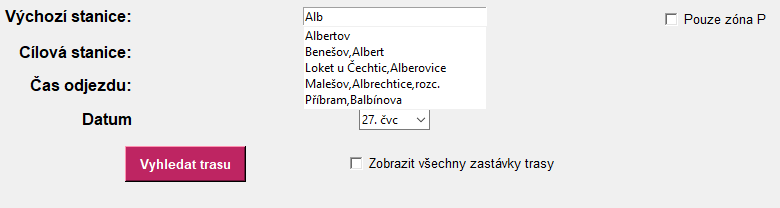
\includegraphics[width = 0.95\textwidth]{gui.png}
		\caption{Základní režim, ve kterém jsou na výběr zastávky ze všech zón.}
        \label{guiAll}
	\end{subfigure}

	\vspace{1em}
	
	\begin{subfigure}[b]{1\textwidth}
		\centering
		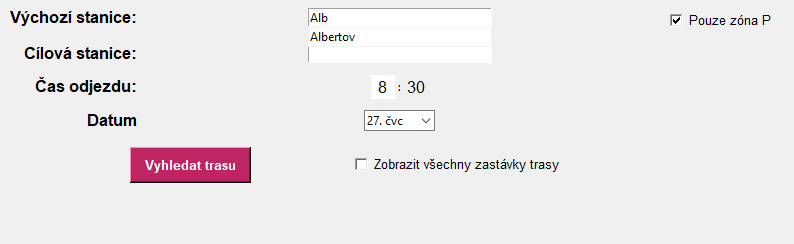
\includegraphics[width = 0.95\textwidth]{guiZonaP.png}
		\caption{Režim, ve kterém jsou na výběr pouze zastávky v~zóně P.}
        \label{guiZoneP}
	\end{subfigure}

	\caption{Zobrazení výběru parematrů trasy v~grafickém uživatelském rozhraní.}
	\label{gui}
\end{figure}

Při zmáčknutí tlačítka \textquote{Vyhledat trasu} se spustí algoritmus TD-Dijkstra s~pareto-optimálními cestami. Všechny pareto-optimální cesty jsou zobrazeny uživateli v~grafickém rozhraní (viz \autoref{guiVypis}). Navíc je zobrazena ještě druhá sada výsledků, u~nichž je čas odjezdu o~půl hodiny posunut v~čase dopředu. Nejedná se o~profilové cesty, protože ty nejsou modifikovány pro pareto řešení, a~tak algoritmus nalezne a~vypíše dvě cesty s~nejdřívějším příjezdem s~odlišným časem odjezdu. U~cest jsou ve výchozím režimu zobrazeny pouze počáteční a~koncové zastávky každé spoje, ale existuje možnost přepnout se do režimu, ve kterém jsou vypsány všechny mezilehlé zastávky.

\begin{figure}[htbp]
	\centering
	\centering
	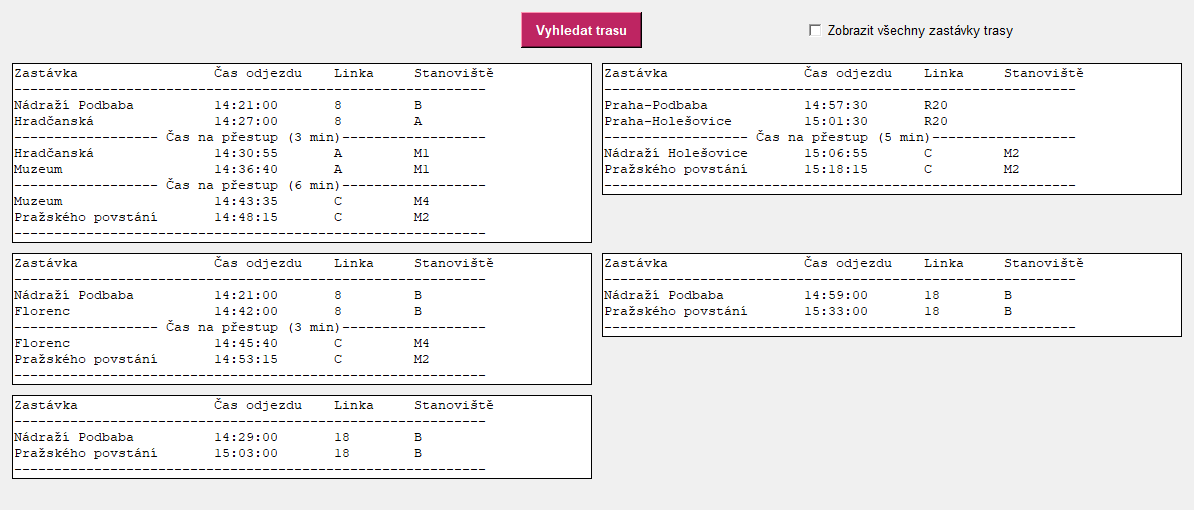
\includegraphics[width = 1.24\textwidth, angle=90, origin =c]{guiVypis.png}
	\caption[Ukázka nalezené množiny pareto-optimálních tras v~grafickém uživatelském rozhraní.]{Ukázka nalezené množiny pareto-optimálních tras v~grafickém uživatelském rozhraní pro výchozí stanici: Nádraží Podbaba, koncovou stanici: Pražského povstání, v~čase 14:20, dne 14.~6.}
	\label{guiVypis}
\end{figure}

\chapter{Výkonnostní testy}
\label{vykonTest}
Algoritmy jsou hodnoceny podle různých kritérií. I~když výsledek dvou algoritmů je totožný, každý z~nich se může uplatnit v~trochu jiných situacích. Na algoritmy vybudované v~této práci (TD-Dijkstra, jeho nástavby a~CSA) se mohou aplikovat tato hodnotící kritéria: korektnost (správnost), časová a~prostorová složitost, doba pre-processingu či flexibilita. Pro tuto práci je dostačující provést pouze test časové složitosti – tj.~jak rychle algoritmus nalezne optimální řešení – ale je nutné počítat s~tím, prostorová složitost může mít vlit na celkovou rychlost algoritmu. K~výchylce algoritmů od korektního (optimálního) řešení dochází u~algoritmů pouze výjimečně.\footnote{Ve velmi vzácných případech ($< 0,1~\%$) může hodnota heuristiky A* přecenit skutečnou vzdálenost (viz \autoref{eukleidMetr}). U~algoritmu ALT dochází k~výraznější odchylce (více než 10 min) přibližně ve 2~\% dotazů. Nepřesnost je pravděpodobně způsobena neidentifikovanou chybou v~implementaci výpočtu cest k~landmarkům a~zpět. Ačkoli je potřeba tuto skutečnost zohlednit při interpretaci výsledků, hlavní závěry této kapitoly zůstávají prakticky neměnné.} Odlišná doba pre-processingu je jen u~ALT algoritmu. Flexibilita je poměrně subjektivní kritérium, které ale má své opodstatnění v~některých aplikacích algoritmů.

\section{Specifikace měřicího zařízení}
Testy výkonu byly provedeny na následující konfiguraci zařízení:

\begin{itemize}
	\item Procesor: Intel Core i5-1135G7 @ 2.40GHz
	\item Operační paměť: 8 GB DDR4
	\item Operační systém: Windows 10 (64-bit)
	\item Programovací jazyk: Python 3.12.1
\end{itemize}

Testy algoritmů neprobíhaly za přísných podmínek, ale za běžného provozu a~bez speciálních optimalizací. U~TD-Dijkstry je použita prioritní fronta knihovny \texttt{heapq}. 

\section{Parametry dopravní sítě}
\renewcommand{\sectionautorefname}{oddíl}
Testování probíhá na dopravní síti VHD v~Praze a~okolí. Data jízdních řádů veřejně zpřístupňuje Pražská integrovaná doprava (PID) (viz \autoref{opendata}). Jízdní řády obsahují kolem 7~700 stanic a~16~700 stanovišť zastávek, které jsou obsluhovány 81~tis. spoji. Celkově jízdní řády obsahují 1,6~milionů spojení (v~průměru 20 na jeden spoj).
\renewcommand{\sectionautorefname}{oddíle}

Samotný graf pro TD-Dijkstru obsahuje přibližně 140 tis. vrcholů (staniční a~linkové dohromady) a~hran je téměř trojnásobek.

\section{Metodika}
Testování algoritmu proběhlo ve dvou režimech, \begin{enumerate*}
	\item[i)] náhodný,
	\item[ii)] zóna P.
\end{enumerate*} 

V náhodném režimu byly kompletně náhodně zvoleny počáteční i~cílové stanice. V~režimu zóna P se vždy alespoň jedna ze stanic nachází v~zóně P; druhá stanice byla zvolena náhodně, tzn.~že výjimečně opět v~zóně P. Výchozí čas byl pro všechny dotazy stanoven na 6:00 a~jednalo se o~běžný pracovní den. 

Měření rychlosti algoritmu probíhá u~TD-Dijkstry ve třech variantách a~pak ve standardní verzi CSA. V~prvním případě se jedná o~základního TD-Dijkstru, A* modifikaci s~Eukleidovskou metrikou a~ALT modifikaci. A* má nastavenou heuristiku jako vzdálenost dělenou 54~km/h (15~m/s). Landmarky se ještě dělí dle způsobu výběru landmarků (\textit{farthest} a~\textit{random}) a~počtu landmarků (8, 16, 32). 

Testování probíhalo na stejných datech napříč režimy: v~rámci jednoho režimu využívaly všechny varianty stejnou sadu počátečních i~cílových stanic. V~obou režimech byla každá varianta algoritmu spuštěna 1000-krát. 

U TD-Dijkstry je měřena Úloha nejdřívějšího příjezdu (nehledě na počet přestupů). U~CSA je také měřena Úloha nejdřívějšího příjezdu, ale zohledňuje se počet přestupů jako sekundární kritérium. Nemělo by to však mít výrazný dopad na časovou složitost.

Výstup měření je medián a~průměr. Medián je vhodný proto, že udává, jak dlouho trvá typický dotaz. Průměr naopak indikuje, jaká je očekávána doba trvání dotazu. Do času vyhledání jedné trasy se počítá i~nalezení trasy, avšak původní načtení hran grafu i~doba pre-processingu u~ALT je z~měření pro přehlednost vyjmuta.

\section{Výsledky}
Výsledky jsou zaznamenány zvlášť pro náhodný výběr stanic a~pro výběr stanic, z~nichž alespoň jedna leží v~zóně P. Očekává se, že u~toho mírně omezeného výběru budou rychlosti algoritmů vyšší, protože nabídka relací z~okolních měst do Prahy je typicky obsáhlejší než u~tangenciálních relací. Cestující tak dorazí do cíle dříve, a~tudíž algoritmus nemusí prozkoumávat tak velkou oblast v~případě TD-Dijkstry anebo vysoký počet spojení u~CSA. Navíc cesta s~nejdřívějším příjezdem u~náhodného výběru často Prahou projíždí anebo je minimálně využit hlavní přestupní terminál, což v~porovnání s~druhým výběrem délku jízdy v~průměru prodlužuje.

Toto očekávání bylo zcela naplněno, protože pro každou variantu platí, že její hodnoty mediánu jsou skoro téměř vždy dvakrát vyšší u~náhodného výběru než u~zóny P. U~průměru jsou hodnoty u~výběru zóna P o~30~\% nižší než u~náhodného výběru.

V \autoref{tab:comp_times_random} jsou vidět hodnoty mediánu i~průměru pro všech 9 variant náhodného výběru. U~žádné z~nich nedošlo k~překročení hranice 1 sekundy. U~náhodného výběru dat je na první pohled vidět, že základní verze algoritmu je nejpomalejší, a~tak praxe potvrzuje, co teoretické poznatky z~předešlých kapitol predikují.

\newcolumntype{L}[1]{>{\raggedleft\arraybackslash}{#1cm}}
\shorthandoff{-}
\renewcommand{\arraystretch}{1.2}
{\small
\begin{table}[ht]
	\centering
		\begin{tabular}{
			>{\raggedright\arraybackslash}m{1.52cm}
			>{\centering\arraybackslash}m{0.78cm}
			>{\centering\arraybackslash}m{0.78cm}
			>{\centering\arraybackslash}m{0.78cm}
			>{\centering\arraybackslash}m{0.78cm}
			>{\centering\arraybackslash}m{0.78cm}
			>{\centering\arraybackslash}m{0.78cm}
			>{\centering\arraybackslash}m{0.78cm}
			>{\centering\arraybackslash}m{0.78cm}
			>{\centering\arraybackslash}m{0.78cm}}
			\toprule
			& \multicolumn{2}{c}{TD-Dijkstra}& \multicolumn{3}{c}{ALT (random)} &\multicolumn{3}{c}{ALT (farthest)} & \\\cmidrule(lr){2-3}\cmidrule(lr){4-6}\cmidrule(lr){7-9}
			& Zákl.&A* & 8 & 16 & 32 & 8 & 16 & 32 & CSA \\
			\midrule
			Medián\thinspace(s)            & 0{,}936 & 0{,}754 & 0{,}593 & 0{,}576 & 0{,}566 & 0{,}597 & 0{,}581 & 0{,}563 & 0{,}600 \\
			Průměr\thinspace(s)             & 0{,}883 & 0{,}813 & 0{,}635 & 0{,}607 & 0{,}609 & 0{,}646 & 0{,}613 & 0{,}610 & 0{,}711 \\
			Relativní medián   & 1{,}00  & 0{,}80  & 0{,}63  & 0{,}62  & 0{,}60  & 0{,}64  & 0{,}62  & 0{,}60  & 0{,}64 \\
			Relativní průměr   & 1{,}00  & 0{,}92  & 0{,}72  & 0{,}69  & 0{,}69  & 0{,}73  & 0{,}69  & 0{,}69  & 0{,}81 \\
			\bottomrule
		\end{tabular}
	\caption[Srovnání rychlostí TD-Dijkstry a~CSA u~dotazů cest s~náhodným výběrem stanic.]{Srovnání rychlostí variací TD-Dijkstry (základní, A* a~ALT) a~CSA u~dotazů cest s~náhodným výběrem stanic. Medián a~průměr je v~sekundách. Také je zobrazena relativní rychlost algoritmů vůči základnímu TD-Dijkstrovi. Slovo v~závorce u~ALT indikuje způsob vybírání landmarků, číslo v~záhlaví jejich počet; v~době trvání není zahrnuta doba předzpracování.}
	\label{tab:comp_times_random}
\end{table}
}

Druhá nejpomalejší varianta je A* s~Eukleidovskou metrikou, která je o~19,5~\% rychlejší než základní TD-Dijkstra podle mediánu a~o~7,9~\% podle průměru. Znamená to, že typický dotaz je zodpovězen znatelně rychleji, ale pravděpodobně kvůli výraznému šikmému rozdělení dat je očekávaná doba vyhledání cesty u~A* jen o~trochu kratší.

Dle výsledků je varianta ALT z~implementovaných algoritmů TD-Dijkstry nejefektivnější, ale mezi jednotlivými verzemi ALT algoritmu jsou jen nepatrné rozdíly. Ve všech z~nich je hodnota mediánu nižší než u~průměru, i~když ne výrazně. Nejlepší z~těchto 6 verzí je ALT s~metodou \textit{farthest} se 32 landmarky, kde činí medián 0,563~s~a~průměr 0,610~s. Existuje malá indikace, že vyšší počet landmarků zvyšuje rychlost algoritmu; každý landmark ale navíc přínáší početní operace, které algoritmus musí provést, a~tak od určitého počtu landmarků užitek z~potenciálně přesnějšího dolního odhadu tuto ztrátu nevykompenzuje.\footnote{Kromě toho vyšší počet landmarků vyžaduje delší čas na pre-processing, ale to je u~velikosti tohoto grafu poměrně zanedbatelný problém, protože u~32 landmarků neoptimalizovaný pre-processing trvá jen několik jednotek minut.}

Mezi metodami \textit{random} a~\textit{farthest} zdá se není rozdíl v~rychlosti algoritmu, což je v~souladu s~\cite{goldberg05PointToPoint}, kde autoři na podobnou věc ve statických grafech poukázali.

V neposlední řadě je negrafový algoritmu Connection Scan Algorithm, u~kterého je hodnota mediánu o~pár setin vyšší než u~ALT, avšak průměr je až o~0,1 s~vyšší než u~\textit{farthest} 32. Očekávané zrychlení, prezentováno např. v~\cite{dibbelt2017CSA}, se nedostavilo. 


{\small
\begin{table}[ht]
	\centering
		\begin{tabular}{
			>{\raggedright\arraybackslash}m{1.52cm}
			>{\centering\arraybackslash}m{0.78cm}
			>{\centering\arraybackslash}m{0.78cm}
			>{\centering\arraybackslash}m{0.78cm}
			>{\centering\arraybackslash}m{0.78cm}
			>{\centering\arraybackslash}m{0.78cm}
			>{\centering\arraybackslash}m{0.78cm}
			>{\centering\arraybackslash}m{0.78cm}
			>{\centering\arraybackslash}m{0.78cm}
			>{\centering\arraybackslash}m{0.78cm}}
			\toprule
			& \multicolumn{2}{c}{TD-Dijkstra}& \multicolumn{3}{c}{ALT (random)} &\multicolumn{3}{c}{ALT (farthest)} & \\\cmidrule(lr){2-3}\cmidrule(lr){4-6}\cmidrule(lr){7-9}
			& Zákl.&A* & 8 & 16 & 32 & 8 & 16 & 32 & CSA \\
			\midrule
			Medián\thinspace(s)       & 0{,}460 & 0{,}369 & 0{,}270 & 0{,}239 & 0{,}213 & 0{,}280 & 0{,}239 & 0{,}239 & 0{,}383 \\
			Průměr\thinspace(s)       & 0{,}583 & 0{,}549 & 0{,}417 & 0{,}394 & 0{,}385 & 0{,}426 & 0{,}399 & 0{,}394 & 0{,}529 \\
			Relativní medián & 1{,}00  & 0{,}80  & 0{,}59  & 0{,}52  & 0{,}46  & 0{,}61  & 0{,}52  & 0{,}52  & 0{,}83 \\
			Relativní průměr & 1{,}00  & 0{,}94  & 0{,}72  & 0{,}68  & 0{,}66  & 0{,}73  & 0{,}68  & 0{,}68  & 0{,}91 \\
			\bottomrule
		\end{tabular}
	\caption[Srovnání rychlostí TD-Dijkstry a~CSA u~dotazů cest, kde je alespoň jedna stanice v~zóně P.]{Srovnání rychlostí variací TD-Dijkstry (základní, A* a~ALT) a~CSA u~dotazů cest, kde je alespoň jedna stanice v~zóně P. Popis tabulky jako v~\autoref{tab:comp_times_random}}
	\label{tab:comp_times_fromP}.
\end{table}
}

\renewcommand{\arraystretch}{1}

V \autoref{tab:comp_times_fromP} je režim zóny P. Jak bylo zmíněno, absolutní hodnoty jsou až dvakrát nižší než u~náhodného výběru. Pro lepší orientaci jsou přidány i~relativní hodnoty mediánu a~průměru. Ty prozrazují, že viditelné rozdíly jsou pouze u~mediánů ALT a~CSA a~u~průměru CSA. Zřejmě tento režim nabízí více \textquote{pěkných} dotazů, které nejsou napříč Středočeským krajem, a~tak heuristiky efektivněji navádí algoritmus do cíle. Nejhorší zhoršení je u~CSA, který je nyní na úrovni A*, což je dáno možná tím, že absence heuristiky zrychluje CSA pouze lineárně, zatímco ostatní algoritmy jsou zrychleny superlineárně.

Verze ALT algoritmu zde benefitují více z~většího množství landmarků, avšak \textit{random} i~\textit{farthest} jsou vesměs srovnatelné. \textit{Random} 32 je zde nejrychlejší; typický dotaz trvá zodpovědět pouze 213~ms.

\section{Diskuze}
Obecně se ukázalo, že ALT je alespoň na určitých vstupech bezkonkurenční v~rámci algoritmů implementovaných v~této práci, ale u~náhodného výběru je na podobné rychlostní úrovni i~CSA. I~jednoduchá Eukleidovská technika zrychluje algoritmus až o~20~\% u~mediánu; benefit u~průměru je mnohem nižší. To samé platí i~u~CSA, u~kterého to může pramenit z~toho, že v~případě zvolení počáteční stanice, ze které v~daný den neodjíždí žádné spoje (protože jezdí např. jenom o~víkendu), CSA musí prohledat celý seznam spojení, od 6 hodin až do ranních hodin dalšího dne. Naopak TD-Dijkstra okamžitě ukončuje vyhledávání. Tím jak je CSA konstruován, při pozdějším čase odjezdu (např. 22:00) by počet spojení k~prohledání byl nižší, a~tudíž i~nižší čas potřebný k~ukončení algoritmu.

Do budoucna se nabízí vyzkoušet i~další metody výběru landmarků, které slibují větší zrychlení za cenu komplikovanějšího a~časově náročnějšího pre-processingu. Také je vhodné nadále experimentovat s~ještě vyšším počtem landmarků za účelem nalezení rovnováhy mezi stále užitečnými odhady a~nepříliš vysokým počtem operací nad landmarky. Výsledky CSA algoritmů indikují, že v~určitých situacích by mohl mít své využití.

\chapter{Závěr}
Tato kapitola shrnuje celý obsah práce a~výsledky vlastních výkonnostních testů algoritmů. Obsahuje i~doporučení pro navazující teoretický a~aplikovaný výzkum.

\section{Shrnutí výsledků práce}
V této práci jsem zhodnotil existující algoritmy na vyhledávání nejrychlejší cest v~jízdních řádech. Dva z~nich, Time-Dependent Dijkstra algoritmus (TD-Dijkstra) a~Connection Scan Algorithm (CSA), jsem naprogramoval v~programovacím jazyku Python a~adaptoval jsem je pro jízdní řády reálného dopravního systému Pražské integrované dopravy (PID). TD-Dijkstra běží ve stanicovém modelu grafu, ve kterém jsou ohodnocení hran proměnlivá. Ohodnocení se mění dle příchodu cestujícího na zastávku a~doby čekání na další spoj. 

CSA, narozdíl od TD-Dijkstry, není grafový algoritmus, ale je založený na postupném průchodu seznamu všech spojení seřazených dle času odjezdu. Dosažitelná spojení upravují ohodnocení nejdřívějšího času příjezdu do stanice.

Existuje mnoho nástaveb pro TD-Dijkstru, které zkracují dobu trvání běhu algoritmu, a~tak jsem i~já některé z~nich aplikoval. Zaprvé se jedná o~A* algoritmus, který při ohodnocování vrcholů pracuje s~heuristikou Eukleidovské metriky převedené na čas. Zadruhé je to ALT algoritmus, který využívá tzv.~landmarků a~principu trojúhelníkové nerovnosti. Heuristika je sice přesnější, což algoritmus zrychluje, ale ALT vyžaduje fázi předzpracování. Tato fáze nicméně u~použitých PID dat není nikterak dlouhá. 

TD-Dijkstra je schopný vypočítat úlohu nejdřívějšího příjezdu do stanice, ale i~kombinovanou úlohu, ve které počet přestupů figuruje jako rovnocenné kritérium. Cestující si tak může sám zvolit, jestli preferuje přijet co nejdříve, anebo později ale s~méně přestupy. U~CSA je počet přestupů pouze sekundární kritérium v~případě stejného času příjezdu.

Prakticky bylo zjištěno, že ALT algoritmy dominují ostatním algoritmům implementovaným v~této práci. Zodpovězení náhodných dotazů trvá něco málo přes půl sekundy (stejně jako u~CSA), zatímco u~základního TD-Dijkstry je to téměř sekunda. U~více realistických dotazů dokonce typický dotaz trvá zodpovědět jen dvě desetiny sekundy v~případě ALT, u~TD-Dijkstry až dvojnásobek.

\section{Doporučení pro budoucí vývoj}
Tato práce je jen malý vhled do toho, jakým způsobem lze nalézt optimální cestu v~systému veřejné hromadné dopravy. Čas příjezdu a~počet přestupů jsou sice důležitá kritéria, ale to stejné platí zřejmě i~o~tarifu. Navíc někteří cestující potřebují vozidlo, které je uzpůsobené pro invalidní vozík nebo kočárek. Vyhledávač spojení by cestu splňující tyto požadavky měl cestujícímu umět nabídnout.

V průběhu práce byly přestupní doby vnímány jako neměnné, ale v~realitě se přestup mezi zastávkami liší. Přestože data od PID přímo nezadávají, jak dlouhý je mezi zastávkami přestup, šlo by to aproximovat vzdáleností zastávek od sebe a~tím, mezi jakými dopravními módy je přestup uskutečňován. Pro větší variabilitu je rovněž smysluplné povolit pěší přestupy mezi poměrně vzdálenými zastávkami, i~když nespadají pod jeden dopravní uzel.

Dále se samozřejmě nabízí rozšířit portfolium algoritmů a~kombinovat různé heuristiky najednou. Contraction hierarchies nebo RAPTOR se zdá být jako potenciálně silný kandidát na rychlé vyhledávání spojů v~jízdních řádech. 

Co se týče implementovaných algoritmů, CSA by se dalo rozšířit i~na další úlohy včetně pareto-optimálních cest. U~ALT algoritmu je naopak možnost vyzkoušet komplikovanější techniky výběru landmarků, které pravděpodobně povedou k~rychlejšímu dotazování, a~experimentovat s~počtem zvolených landmarků.
